

\chapter{Results}
\label{chapter:results}

In this chapter we will implement all the models described before: constant volatility, Dupire's local volatility, Heston's stochastic volatility and both static and dynamic SABR models.

With the exception of Dupire's local volatility, will perform the calibration described in section \ref{section:Model Calibration} for all models: we will minimize the cost function in eq. \eqref{cost} with the weight function shown in eq. \eqref{weight}. We shall apply both the MultiStart and the CMA-ES optimization algorithms to find the optimal solution.

We will fit all our functions to a dataset of implied volatilities for European options with different maturities and strike prices. This data was kindly provided by \emph{BNP Paribas} and is shown in Appendix \ref{chapter:mktdata}.


For the case of Dupire's local volatility, no calibration is required. Instead we must perform an interpolation in order to find the implied volatility surface from the data mentioned before and, with it, find the local volatility function. From this, we can easily obtain the prices of European options from the Monte Carlo pricer described in subsections \ref{subsection:Simulating stock prices} and \ref{subsection:Pricing options from simulations}. These prices (and their implied volatilities) can then be compared to their true market values.

Some parameters will be used throughout all the simulations, namely the initial stock price, $S_0$, the risk-free interest rate, $r$, and the time step size (used in the Monte Carlo simulations), $\Delta t$. Their values are shown in \autoref{tab:defaultparam}.
\begin{table}[H]
    \centering
        \renewcommand{\arraystretch}{0.8}
\begin{tabular}{@{}lcr@{}}
\toprule
$S_0$($\EUR$) & $r$($\SI{}{\per\year}$) & $\Delta t$(days) \\ \midrule
1 & 0 & 0.5 \\
\bottomrule
\end{tabular}
  \caption[Parameters used throughout all simulations.]{Parameters used throughout all simulations.}
  \label{tab:defaultparam}
\end{table}



\section{Constant Volatility Model}
\begin{figure}[H]
  \begin{subfigmatrix}{2}
    \subfigure[$T=21$ days]{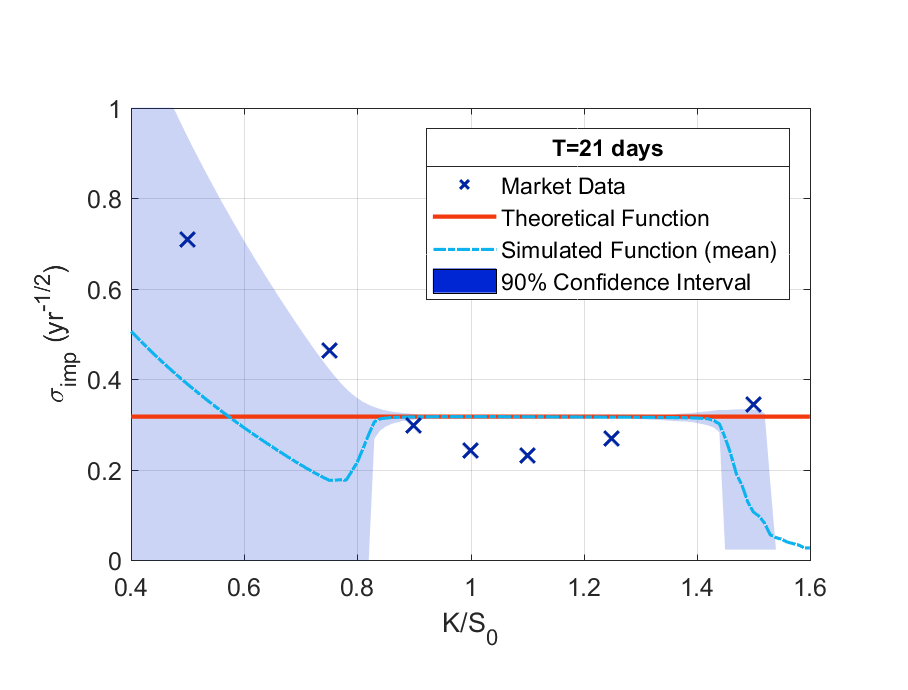
\includegraphics[width=0.49\linewidth,trim={0.25cm 0.45cm 1.1cm 1.4cm},clip]{ConstVol1.eps}}
    \subfigure[$T=42$ days]{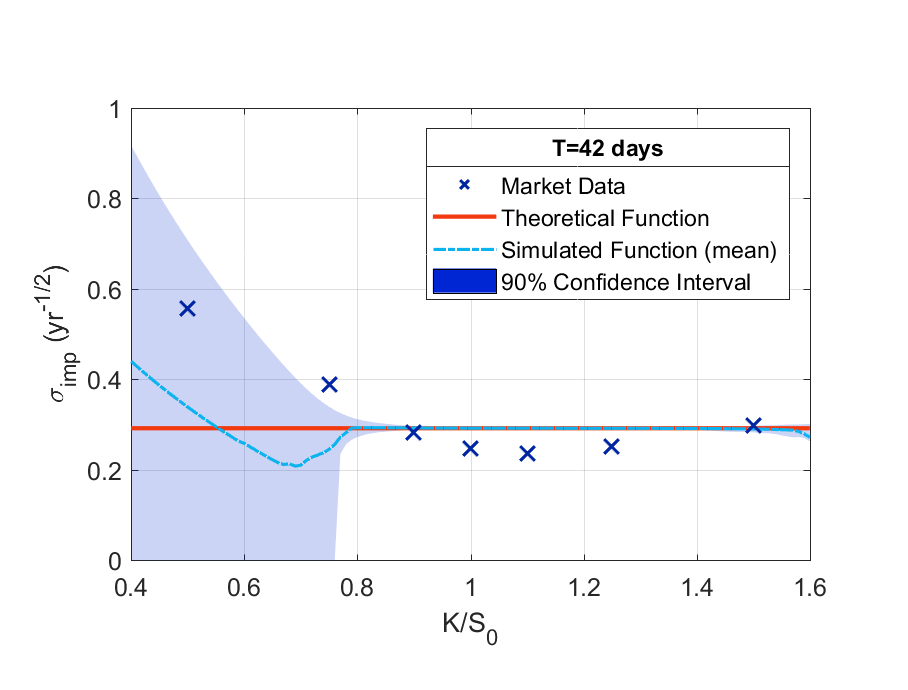
\includegraphics[width=0.49\linewidth,trim={0.25cm 0.45cm 1.1cm 1.4cm},clip]{ConstVol2.eps}}
    \subfigure[$T=63$ days]{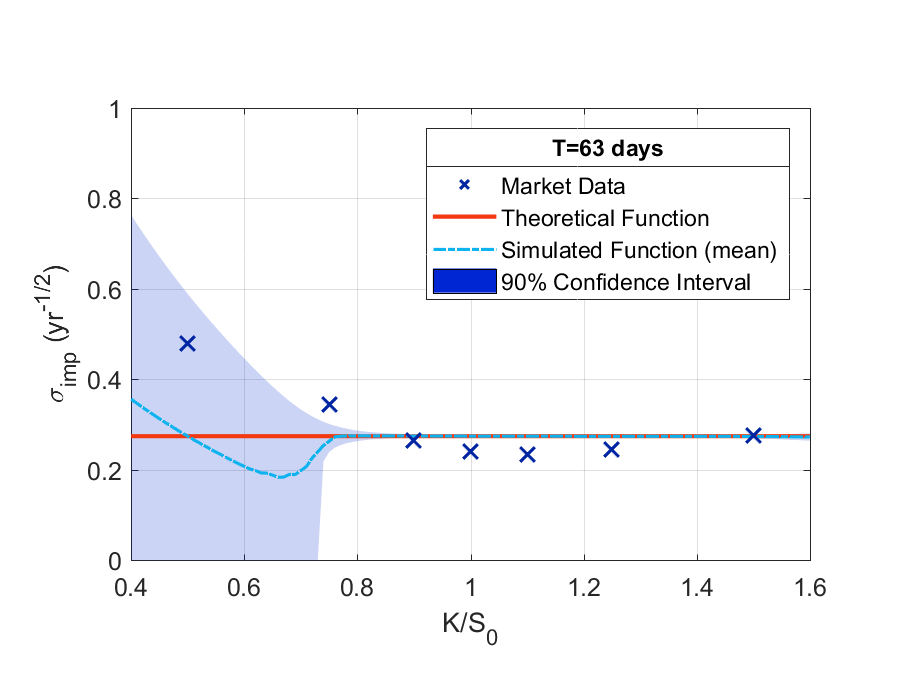
\includegraphics[width=0.49\linewidth,trim={0.25cm 0.45cm 1.1cm 1.4cm},clip]{ConstVol3.eps}}
    \subfigure[$T=126$ days]{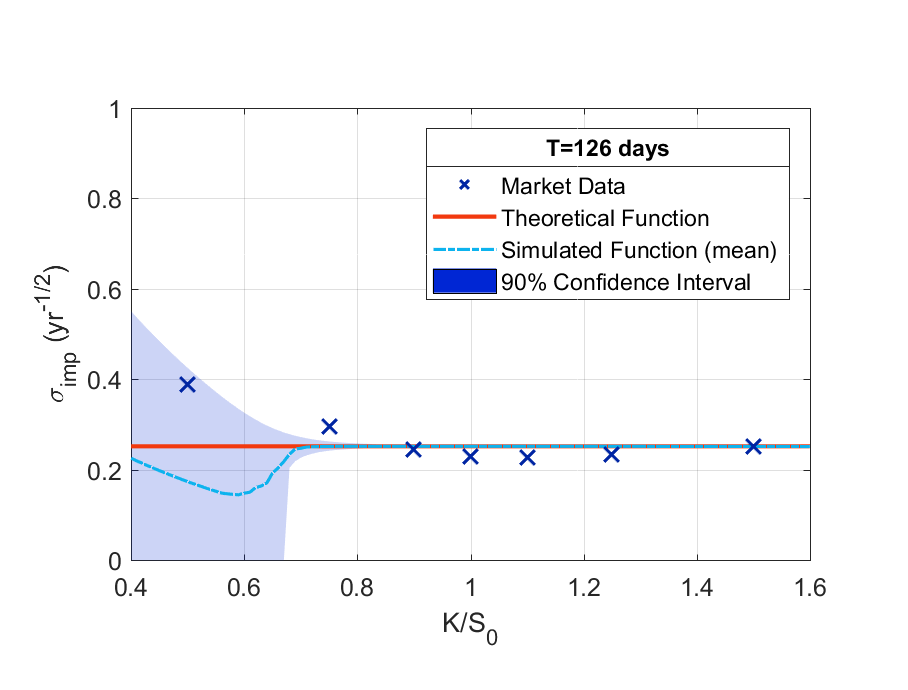
\includegraphics[width=0.49\linewidth,trim={0.25cm 0.45cm 1.1cm 1.4cm},clip]{ConstVol4.eps}}
  \end{subfigmatrix}
  \caption[Implied volatility functions fitted independently to the implied volatility data for different maturities under constant volatility model, plotted with their respective Monte Carlo simulated functions along with their confidence intervals.]{Implied volatility functions (red lines) fitted independently to the implied volatility data (crosses) for different maturities under constant volatility model, plotted with their respective Monte Carlo simulated functions (light-blue dot-dashed lines) along with their 90\% confidence intervals (blue region).}
  \label{fig:ConstVol}
\end{figure}


\begin{table}[H]
    \centering
        \renewcommand{\arraystretch}{0.8}
\begin{tabular}{@{}lcr@{}}
\toprule
$T$ (days) & $\sigma_{imp,\mathrm{mdl}}$ ($\SI{}{\year\tothe{-1/2}}$) & Cost \\ \midrule
21 & 0.3174 & 0.0635 \\
42 & 0.2918 & 0.0282 \\
63 & 0.2742 & 0.0164 \\
126& 0.2518 & 0.0069 \\
\bottomrule
\end{tabular}
  \caption[Fitted parameters for each maturity (fitted independently) under constant volatility model.]{Fitted parameters for each maturity (fitted independently) under constant volatility model.}
  \label{tab:ConstVolPar}
\end{table}


\begin{table}[H]
\centering
\renewcommand{\arraystretch}{0.8}
\begin{tabular}{@{}lccccccr@{}}
\toprule
$T$(days) & $K$($\EUR$) & $\sigma_{i,\mathrm{mkt}}$($\SI{}{\year\tothe{-1/2}}$) &  $\sigma_{i,\mathrm{mdl}}$($\SI{}{\year\tothe{-1/2}}$) &$\mathrm{Error}_{\sigma}(\%)$&$C_{\mathrm{mkt}}$($\EUR$)&$C_{\mathrm{mdl}}$($\EUR$)& \multicolumn{1}{c}{$\mathrm{Error}_{C}(\%)$}\\ \midrule
\multirow{7}{*}{21} & 0.50 & 0.7082 & \multirow{7}{*}{0.3174} & 55.2 & 0.50001 & 0.50000 & 0.003 \\
&0.75 & 0.4632 &  & 31.5 & 0.25065 & 0.25002 & 0.3 \\
&0.90 & 0.2989 &  & 6.2 & 0.10439 & 0.10540 & 1.0 \\
&1.00 & 0.2425 &  & 30.9 & 0.02792 & 0.03654 & 30.9 \\
&1.10 & 0.2314 &  & 37.1 & 2.42$\times10^{-3}$ & 7.41$\times10^{-3}$ & 205.9 \\
&1.25 & 0.2699 &  & 17.6 & 5.34$\times10^{-5}$ & 25.01$\times10^{-5}$ & 367.9 \\
&1.50 & 0.3433 &  & 7.5 & 5.75$\times10^{-7}$ & 1.12$\times10^{-7}$ & 80.5 \\\midrule
\multirow{7}{*}{42}&0.50 & 0.5556 & \multirow{7}{*}{0.2918} & 47.5 & 0.50005 & 0.50000 & 0.01 \\
&0.75 & 0.3876 &  & 24.7 & 0.25186 & 0.25027 & 0.6 \\
&0.90 & 0.2824 &  & 3.3 & 0.11069 & 0.11166 & 0.9 \\
&1.00 & 0.2461 &  & 18.6 & 0.04006 & 0.04749 & 18.5 \\
&1.10 & 0.2354 &  & 23.9 & 8.52$\times10^{-3}$ & 15.00$\times10^{-3}$ & 75.9 \\
&1.25 & 0.2525 &  & 15.6 & 6.21$\times10^{-4}$ & 15.75$\times10^{-4}$ & 153.8 \\
&1.50 & 0.2968 &  & 1.7 & 1.58$\times10^{-5}$ & 1.24$\times10^{-5}$ & 21.4 \\\midrule
\multirow{7}{*}{63}&0.50 & 0.4789 &\multirow{7}{*}{0.2742}  & 42.7 & 0.50009 & 0.50000 & 0.02 \\
&0.75 & 0.3452 &  & 20.6 & 0.25296 & 0.25077 & 0.9 \\
&0.90 & 0.2658 &  & 3.2 & 0.11533 & 0.11650 & 1.0 \\
&1.00 & 0.2401 &  & 14.2 & 0.04787 & 0.05465 & 14.2 \\
&1.10 & 0.2330 &  & 17.7 & 0.01421 & 0.02069 & 45.5 \\
&1.25 & 0.2438 &  & 12.5 & 1.80$\times10^{-3}$ & 3.33$\times10^{-3}$ & 85.1 \\
&1.50 & 0.2749 &  & 0.3 & 7.66$\times10^{-5}$ & 7.44$\times10^{-5}$ & 2.9 \\\midrule
\multirow{7}{*}{126}&0.50 & 0.3878 &  \multirow{7}{*}{0.2518}& 35.1 & 0.50035 & 0.50000 & 0.07 \\
&0.75 & 0.2954 &  & 14.7 & 0.25694 & 0.25344 & 1.4 \\
&0.90 & 0.2444 &  & 3.1 & 0.12716 & 0.12882 & 1.3 \\
&1.00 & 0.2295 &  & 9.7 & 0.06467 & 0.07094 & 9.7 \\
&1.10 & 0.2269 &  & 11.0 & 0.02862 & 0.03488 & 21.9 \\
&1.25 & 0.2340 &  & 7.6 & 7.57$\times10^{-3}$ & 9.98$\times10^{-3}$ & 31.8 \\
&1.50 & 0.2521 &  & 0.1 & 8.58$\times10^{-4}$ & 8.51$\times10^{-4}$ & 0.8 \\
\bottomrule
\end{tabular}
  \caption[Comparison between fitted results and original data under constant volatility model.]{Comparison between fitted functions and original data under constant volatility model.}
  \label{tab:CV}
\end{table}








\newpage
\section{Dupire Model}

\begin{figure}[H]
  \begin{subfigmatrix}{2}
    \subfigure[$\sigma_{imp}$ surface]{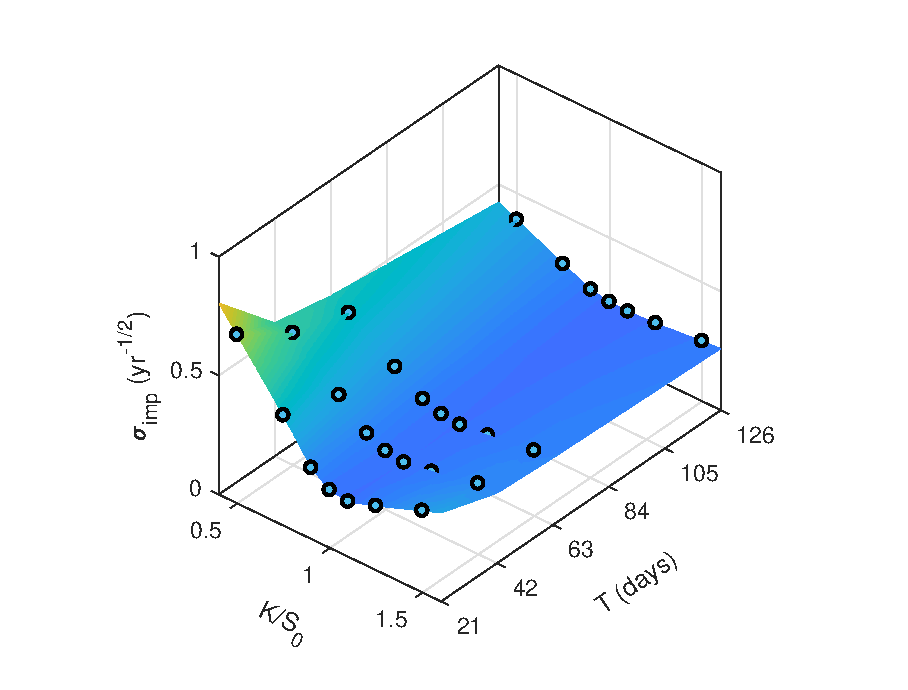
\includegraphics[width=0.49\linewidth,trim={1.7cm 0.45cm 2.35cm 0.85cm},clip]{ImpliedV.eps}}
    \subfigure[$\sigma_{imp}$ contour plot]{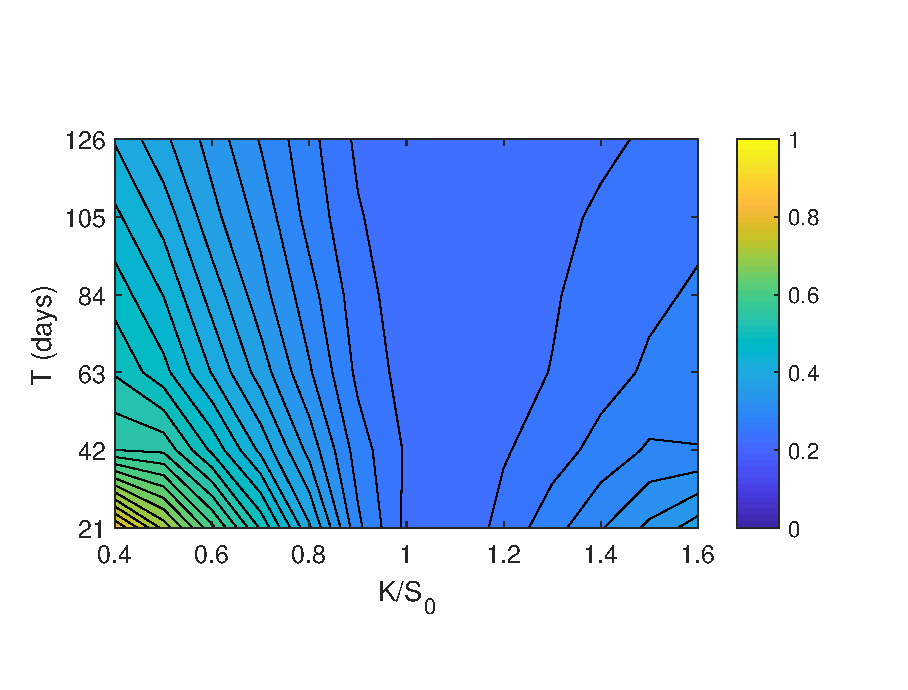
\includegraphics[width=0.49\linewidth,trim={0.2cm 0.5cm 1.25cm 1.55cm},clip]{ImpliedVC.eps}}
  \end{subfigmatrix}
    \caption[Implied volatility surface and corresponding contour plot of the function interpolated linearly between the original data points.]{Implied volatility surface (left) and corresponding contour plot (right) of the function interpolated linearly between the original data points (blue circles).}\label{fig:DupImpV}
\end{figure}   


\begin{figure}[H]
  \begin{subfigmatrix}{2}
    \subfigure[$\sigma_{loc}$ surface]{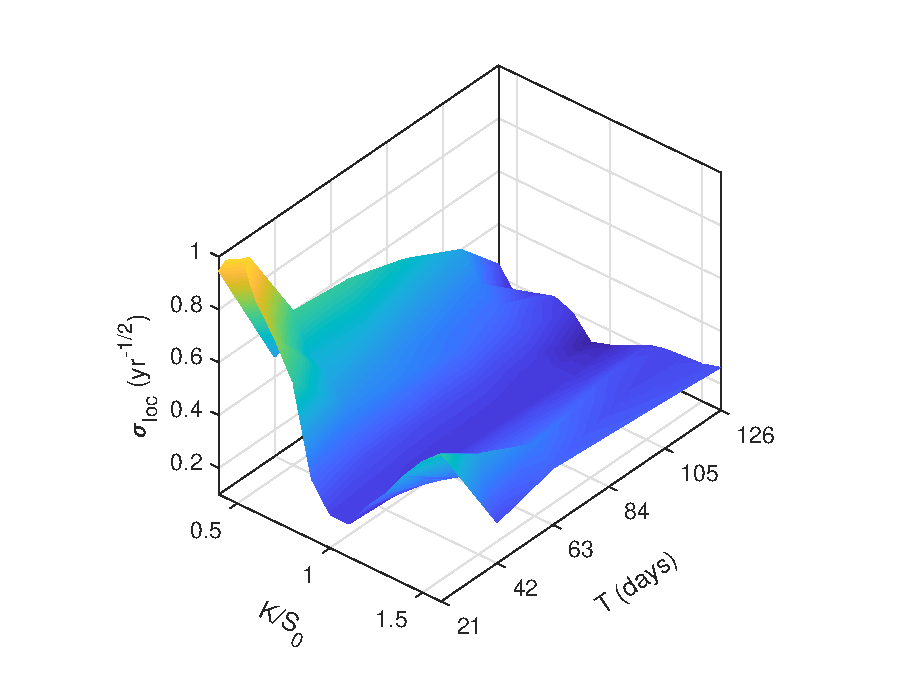
\includegraphics[width=0.49\linewidth,trim={1.7cm 0.45cm 2.35cm 0.85cm},clip]{LocalV.eps}}
    \subfigure[$\sigma_{loc}$ contour plot]{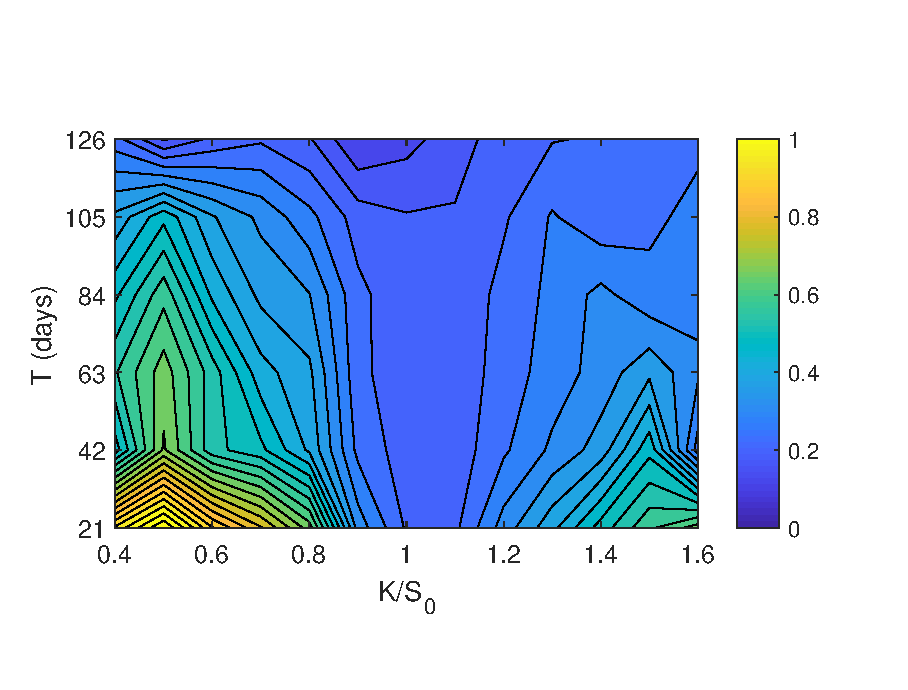
\includegraphics[width=0.49\linewidth,trim={0.2cm 0.5cm 1.25cm 1.55cm},clip]{LocalVC.eps}}
  \end{subfigmatrix}
    \caption[Local volatility surface and corresponding contour plot of the function obtained with Dupire's formula from the interpolated implied volatility surface.]{Local volatility surface (left) and corresponding contour plot (right) of the function obtained with Dupire's formula (eq.\eqref{dupire2}) from the interpolated implied volatility surface in \autoref{fig:DupImpV}.}\label{fig:DupLocVol}
\end{figure}   


\begin{figure}[H]
  \begin{subfigmatrix}{2}
    \subfigure[$T=21$ days]{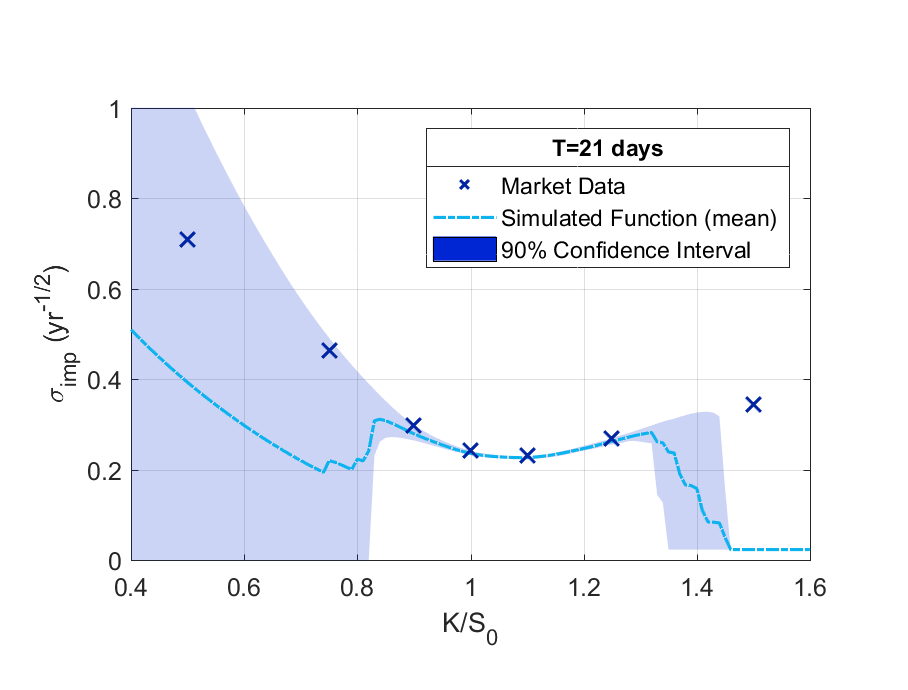
\includegraphics[width=0.49\linewidth,trim={0.25cm 0.45cm 1.1cm 1.4cm},clip]{Dup1.eps}}
    \subfigure[$T=42$ days]{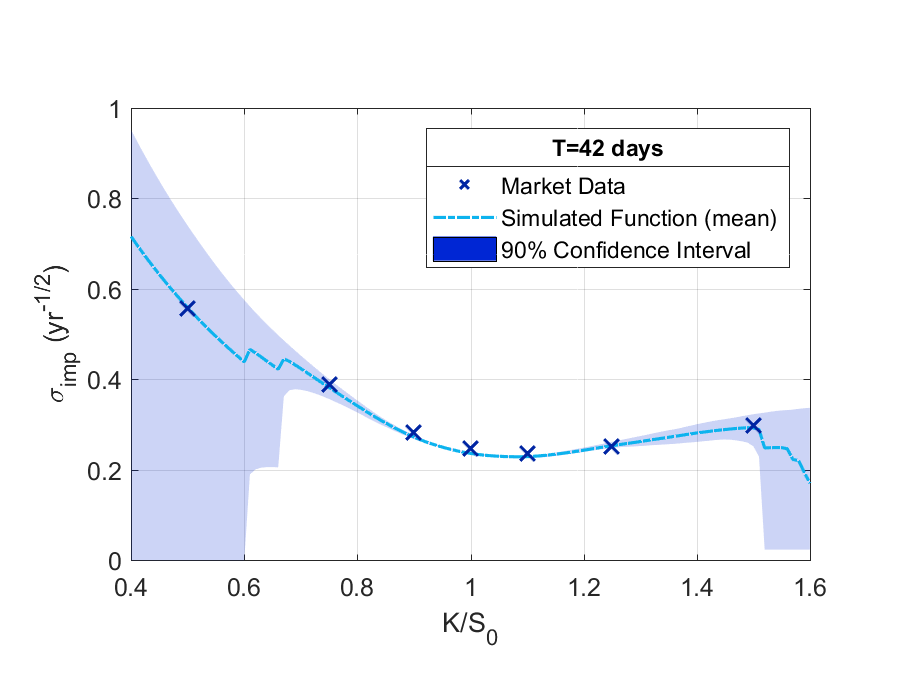
\includegraphics[width=0.49\linewidth,trim={0.25cm 0.45cm 1.1cm 1.4cm},clip]{Dup2.eps}}
    \subfigure[$T=63$ days]{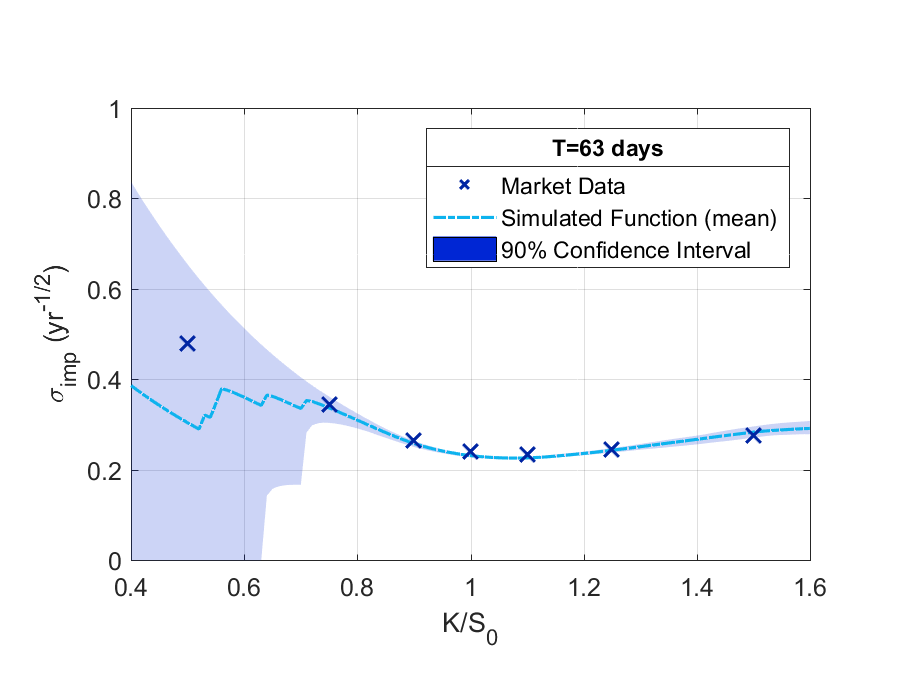
\includegraphics[width=0.49\linewidth,trim={0.25cm 0.45cm 1.1cm 1.4cm},clip]{Dup3.eps}}
    \subfigure[$T=126$ days]{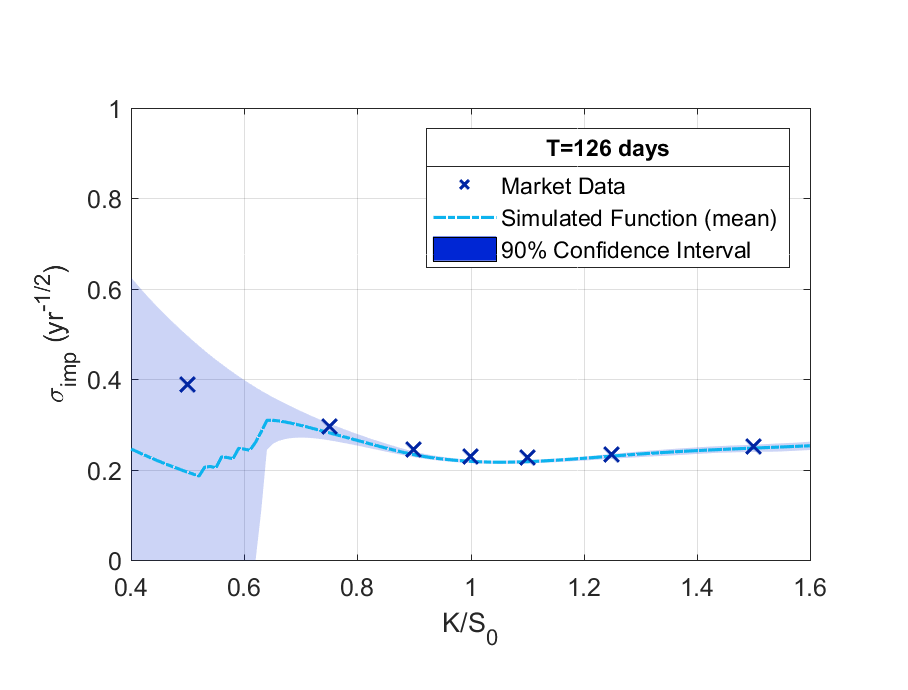
\includegraphics[width=0.49\linewidth,trim={0.25cm 0.45cm 1.1cm 1.4cm},clip]{Dup4.eps}}
  \end{subfigmatrix}
  \caption[Implied volatility functions simulated with Monte Carlo under Dupire's local volatility model with their corresponding 90\% confidence interval, plotted against the original market data.]{Implied volatility functions (light-blue dot-dashed) simulated with Monte Carlo under Dupire's local volatility model with their corresponding 90\% confidence interval, plotted against the original market data (crosses).}
  \label{fig:Dup}
\end{figure}


\begin{figure}[H]
  \begin{subfigmatrix}{2}
    \subfigure[$\sigma_{imp}$ surface]{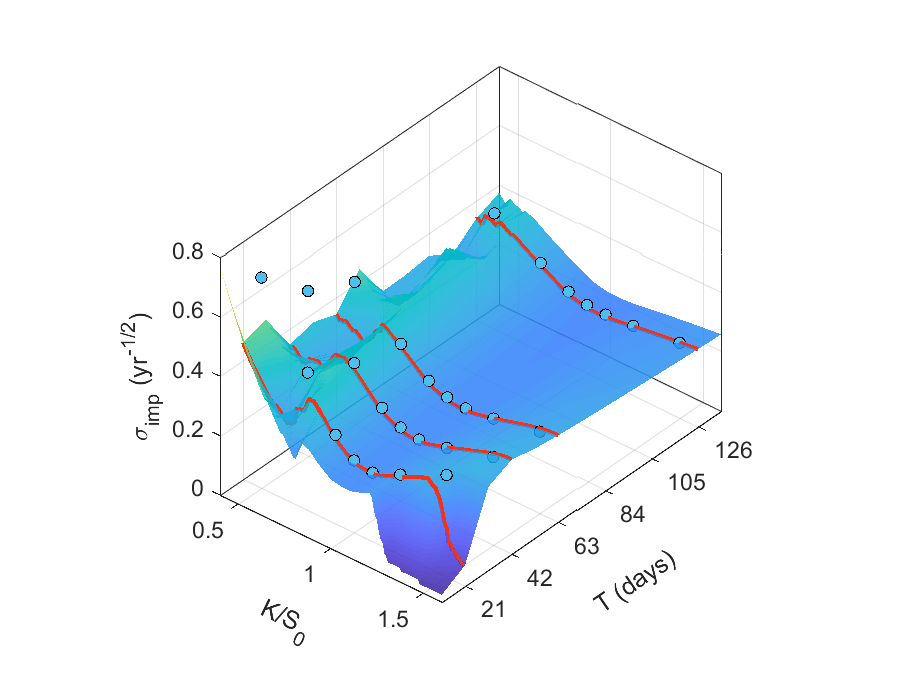
\includegraphics[width=0.49\linewidth,trim={1.7cm 0.45cm 1.9cm 0.85cm},clip]{DupS.eps}}
    \subfigure[$\sigma_{imp}$ contour plot]{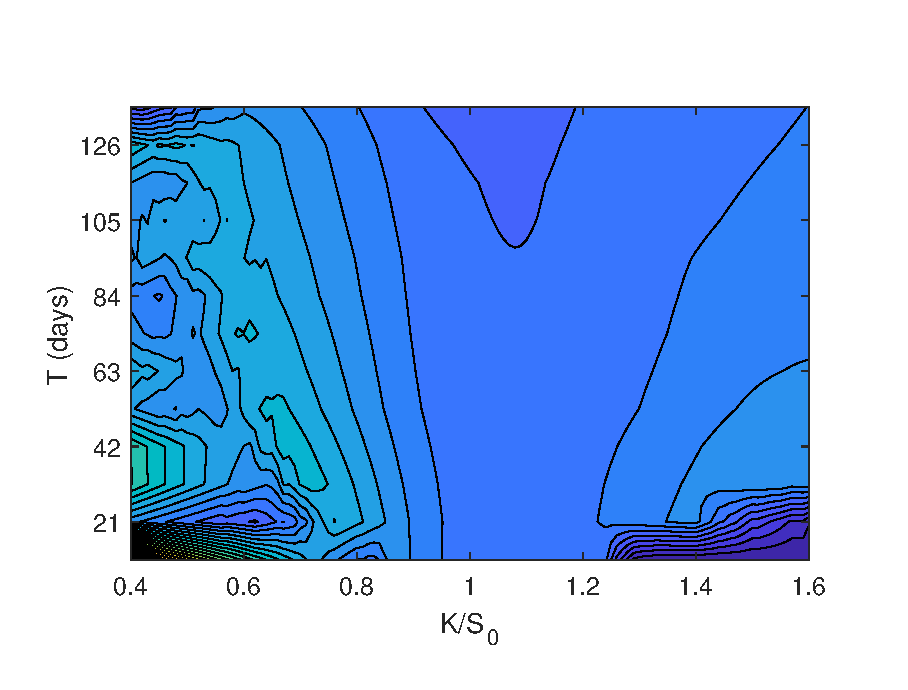
\includegraphics[width=0.49\linewidth,trim={0.2cm 0.5cm 1.25cm 1.55cm},clip]{DupSC.eps}}
  \end{subfigmatrix}
    \caption[Implied volatility surface and corresponding contour plot simulated with Monte Carlo under Dupire's local volatility model plotted against the original market data and the generated functions shown in \autoref{fig:Dup}.]{Implied volatility surface (left) and corresponding contour plot (right) simulated with Monte Carlo under Dupire's local volatility model plotted against the original market data (blue circles) and the generated functions shown in \autoref{fig:Dup} (red dot-dashed lines).}\label{fig:DupS}
\end{figure}   

\begin{table}[H]
    \centering
        \renewcommand{\arraystretch}{0.8}
\begin{tabular}{@{}ccccccccc@{}}
\toprule
\multicolumn{6}{c|}{Interpolation} & \multicolumn{3}{c}{Simulation} \\ \midrule
$T_{min}$(days) & $T_{max}$(days) & $\Delta T$(days) & $K_{min}$($\EUR$) & $K_{max}$($\EUR$) & \multicolumn{1}{c|}{$\Delta K$($\EUR$)} & $N_{paths}$ & $N_{reps}$ & $\sigma_{max}$($\SI{}{\year\tothe{-1/2}}$) \\ \midrule
21 & 126 & 10.5 & 0.4 & 1.6 & \multicolumn{1}{c|}{0.05} & 50000 & 30 & 2 \\ \bottomrule
\end{tabular}
  \caption[Parameters used in the interpolation and simulation sections of Dupire's model.]{Parameters used in the interpolation and simulation sections of Dupire's model.}
  \label{tab:DupR}
\end{table}



\begin{table}[H]
\centering
\renewcommand{\arraystretch}{0.8}
\begin{tabular}{@{}lccccccr@{}}
\toprule
$T$(days) & $K$($\EUR$) & $\sigma_{i,\mathrm{mkt}}$($\SI{}{\year\tothe{-1/2}}$) &  $\sigma_{i,\mathrm{mdl}}$($\SI{}{\year\tothe{-1/2}}$) &$\mathrm{Error}_{\sigma}(\%)$&$C_{\mathrm{mkt}}$($\EUR$)&$C_{\mathrm{mdl}}$($\EUR$)& $\mathrm{Error}_{C}(\%)$\\ \midrule
\multirow{7}{*}{21} & 0.50 & 0.7082 & 0.2319 & 67.3 & 0.50001 & 0.50000 & 0.003 \\
 & 0.75 & 0.4632 & 0.3740 & 19.3 & 0.25065 & 0.25011 & 0.2 \\
 & 0.90 & 0.2989 & 0.2845 & 4.8 & 0.10439 & 0.10368 & 0.7 \\
 & 1.00 & 0.2425 & 0.2374 & 2.1 & 0.02792 & 0.02734 & 2.1 \\
 & 1.10 & 0.2314 & 0.2276 & 1.7 & 2.42$\times10^{-3}$ & 2.26$\times10^{-3}$ & 6.8 \\
 & 1.25 & 0.2699 & 0.2633 & 2.5 & 5.34$\times10^{-5}$ & 4.06$\times10^{-5}$ & 24.0 \\
 & 1.50 & 0.3433 & 0.1421 & 58.6 & 5.75$\times10^{-7}$ & 0 & 100.0 \\\midrule
\multirow{7}{*}{42} & 0.50 & 0.5556 & 0.3846 & 30.8 & 0.50005 & 0.50000 & 0.01 \\
 & 0.75 & 0.3876 & 0.3683 & 5.0 & 0.25186 & 0.25139 & 0.2 \\
 & 0.90 & 0.2824 & 0.2700 & 4.4 & 0.11069 & 0.10946 & 1.1 \\
 & 1.00 & 0.2461 & 0.2358 & 4.2 & 0.04006 & 0.03838 & 4.2 \\
 & 1.10 & 0.2354 & 0.2286 & 2.9 & 8.52$\times10^{-3}$ & 7.83$\times10^{-3}$ & 8.2 \\
 & 1.25 & 0.2525 & 0.2539 & 0.6 & 6.21$\times10^{-4}$ & 6.46$\times10^{-4}$ & 4.1 \\
 & 1.50 & 0.2968 & 0.3089 & 4.1 & 1.58$\times10^{-5}$ & 2.70$\times10^{-5}$ & 70.3 \\\midrule
\multirow{7}{*}{63} & 0.50 & 0.4789 & 0.3176 & 33.7 & 0.50009 & 0.50000 & 0.02 \\
 & 0.75 & 0.3452 & 0.3355 & 2.8 & 0.25296 & 0.25256 & 0.2 \\
 & 0.90 & 0.2658 & 0.2578 & 3.0 & 0.11533 & 0.11424 & 0.9 \\
 & 1.00 & 0.2401 & 0.2310 & 3.8 & 0.04787 & 0.04606 & 3.8 \\
 & 1.10 & 0.2330 & 0.2253 & 3.3 & 0.01421 & 0.01307 & 8.0 \\
 & 1.25 & 0.2438 & 0.2440 & 0.1 & 1.80$\times10^{-3}$ & 1.81$\times10^{-3}$ & 0.5 \\
 & 1.50 & 0.2749 & 0.2845 & 3.5 & 7.66$\times10^{-5}$ & 11.15$\times10^{-5}$ & 45.7 \\\midrule
\multirow{7}{*}{126} & 0.50 & 0.3878 & 0.3870 & 0.2 & 0.50035 & 0.50035 & 0.001 \\
 & 0.75 & 0.2954 & 0.2876 & 2.6 & 0.25694 & 0.25623 & 0.3 \\
 & 0.90 & 0.2444 & 0.2358 & 3.5 & 0.12716 & 0.12528 & 1.5 \\
 & 1.00 & 0.2295 & 0.2203 & 4.0 & 0.06467 & 0.06207 & 4.0 \\
 & 1.10 & 0.2269 & 0.2190 & 3.5 & 0.02862 & 0.02667 & 6.8 \\
 & 1.25 & 0.2340 & 0.2319 & 0.9 & 7.57$\times10^{-3}$ & 7.31$\times10^{-3}$ & 3.4 \\
 & 1.50 & 0.2521 & 0.2528 & 0.3 & 8.58$\times10^{-4}$ & 8.77$\times10^{-4}$ & 2.2 \\
 \bottomrule
\end{tabular}
  \caption[Comparison between the data obtained by generating $N_{paths}$ paths under Dupire's local volatility model using the Monte Carlo pricing method and the original data.]{Comparison between the data obtained by generating $N_{paths}$ paths under Dupire's local volatility model using the Monte Carlo pricing method and the original data.}
  \label{tab:Dup}
\end{table}










\newpage
\section{Static SABR Model}
As we saw before, the Static SABR model is defined as
\begin{equation}
dS=rSdt+e^{-r(T-t)(1-\beta)}\sigma S^\beta dW_1,
\end{equation}
\begin{equation}
d\sigma=\nu\sigma dW_2,
\end{equation}
\noindent with $\alpha=\sigma(0)$ and with $W_1$ and $W_2$ having a correlation of $\rho$.

The closed form solution, shown in eq.\eqref{sabr}, enables us to obtain the theoretical implied volatilities of options priced under this model and will be used in the calibration process.

The influence of each parameter of the Static SABR model on the shape of the implied volatility curve is shown in \autoref{fig:SSparam}.

\begin{figure}[H]
  \begin{subfigmatrix}{2}
    \subfigure[Dependence on $\alpha$]{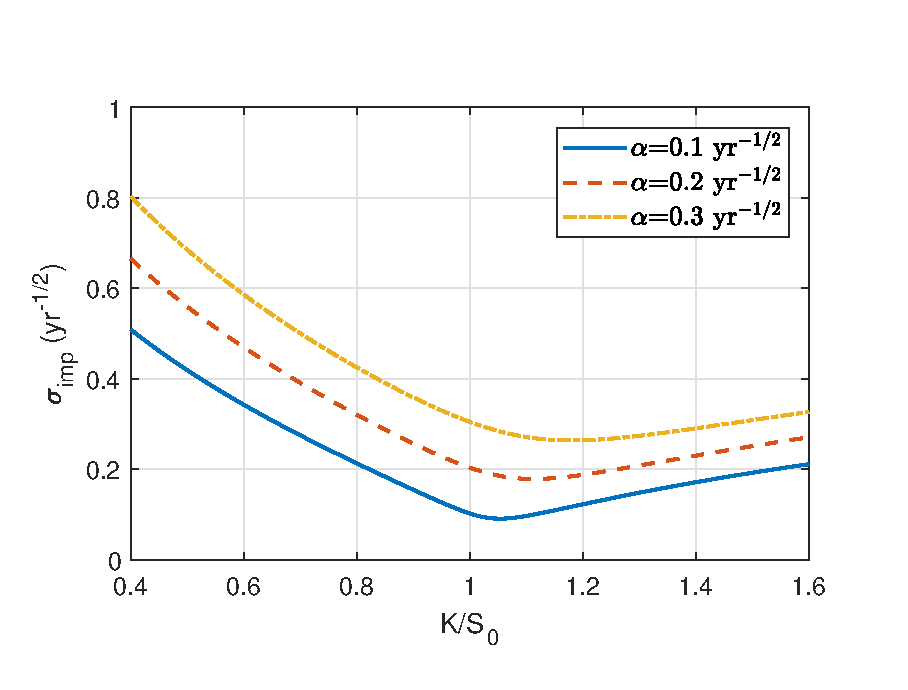
\includegraphics[width=0.49\linewidth,trim={0.25cm 0.45cm 1.1cm 1.4cm},clip]{SSalpha.eps}}
    \subfigure[Dependence on $\beta$]{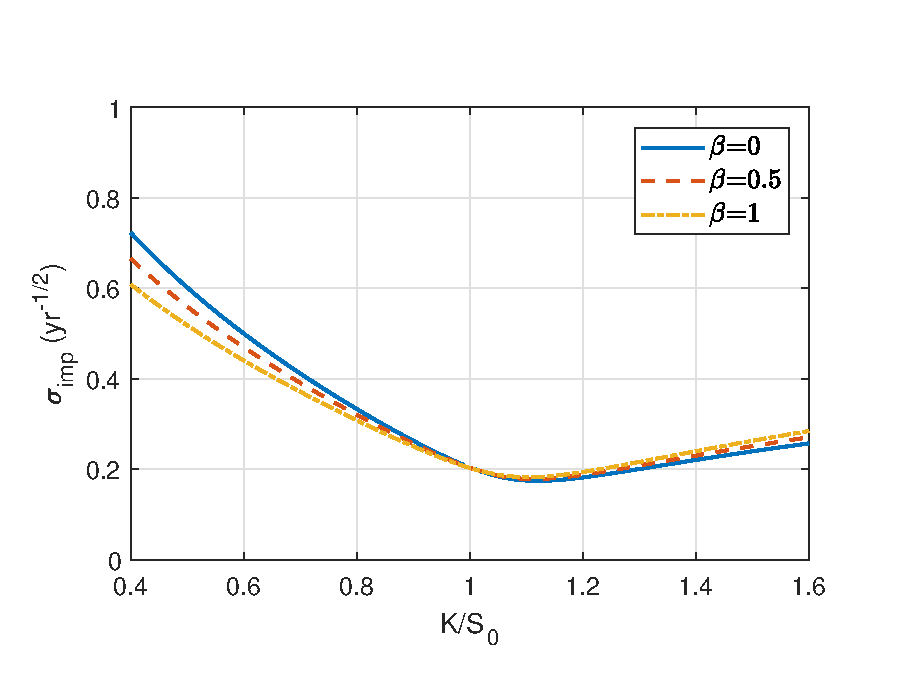
\includegraphics[width=0.49\linewidth,trim={0.25cm 0.45cm 1.1cm 1.4cm},clip]{SSbeta.eps}}
    \subfigure[Dependence on $\rho$]{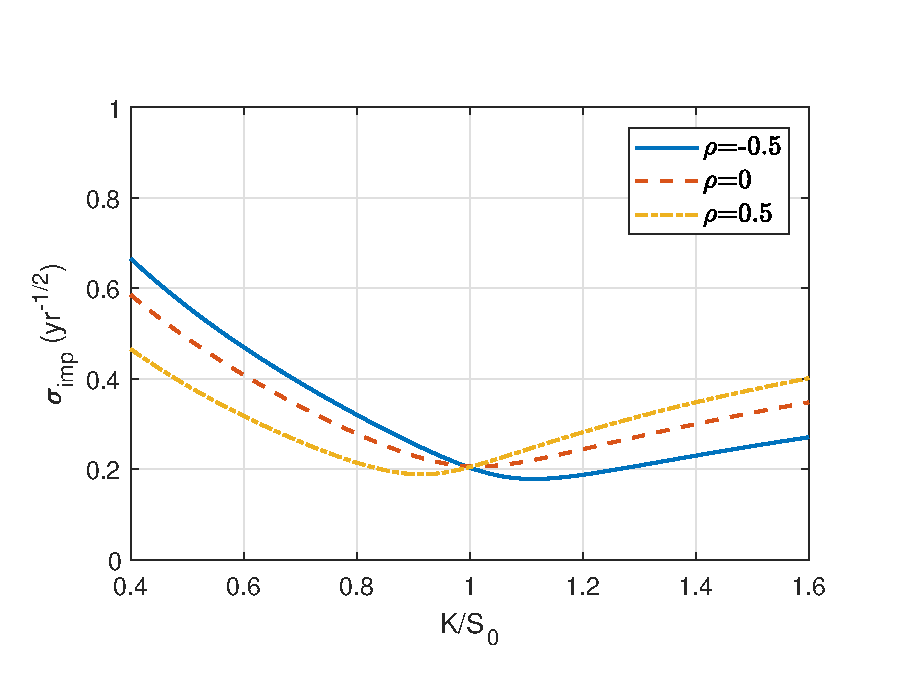
\includegraphics[width=0.49\linewidth,trim={0.25cm 0.45cm 1.1cm 1.4cm},clip]{SSrho.eps}}
    \subfigure[Dependence on $\nu$]{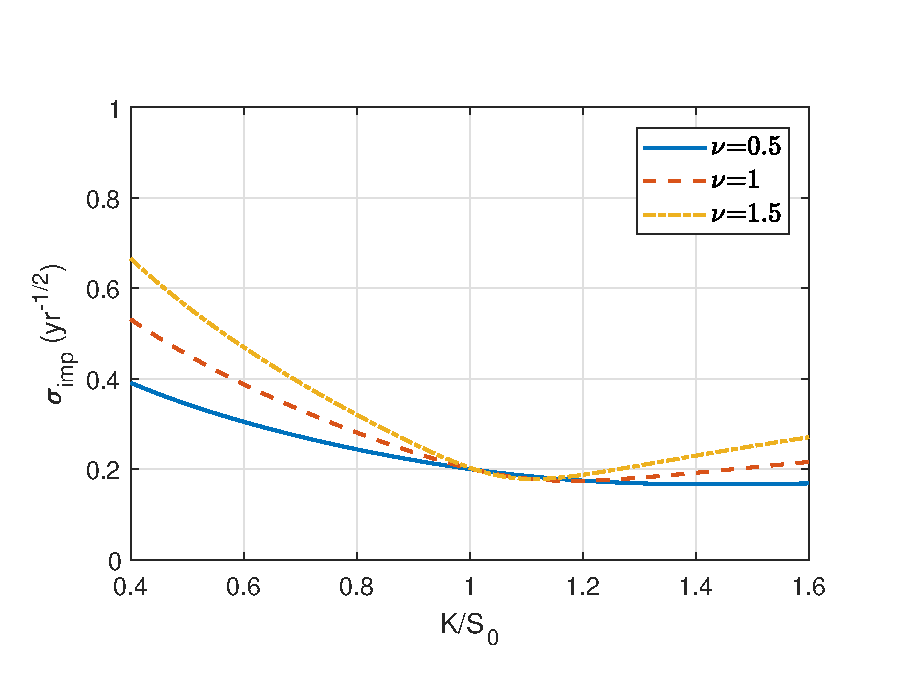
\includegraphics[width=0.49\linewidth,trim={0.25cm 0.45cm 1.1cm 1.4cm},clip]{SSnu.eps}}
  \end{subfigmatrix}
  \caption[Dependence of the implied volatility curve on each of the Static SABR model parameters.]{Dependence of the implied volatility curve on each of the Static model SABR parameters. The default parameters used were $S_0=1\EUR$, $T=42$ days and $r=0$. Furthermore, on all plots, except when the dependence on a parameter is represented, the parameters used were $\alpha=0.2$, $\beta=1$, $\rho=-0.5$ and $\nu=1.5$.}
  \label{fig:SSparam}
\end{figure}


\begin{figure}[H]
  \begin{subfigmatrix}{2}
    \subfigure[$T=21$ days]{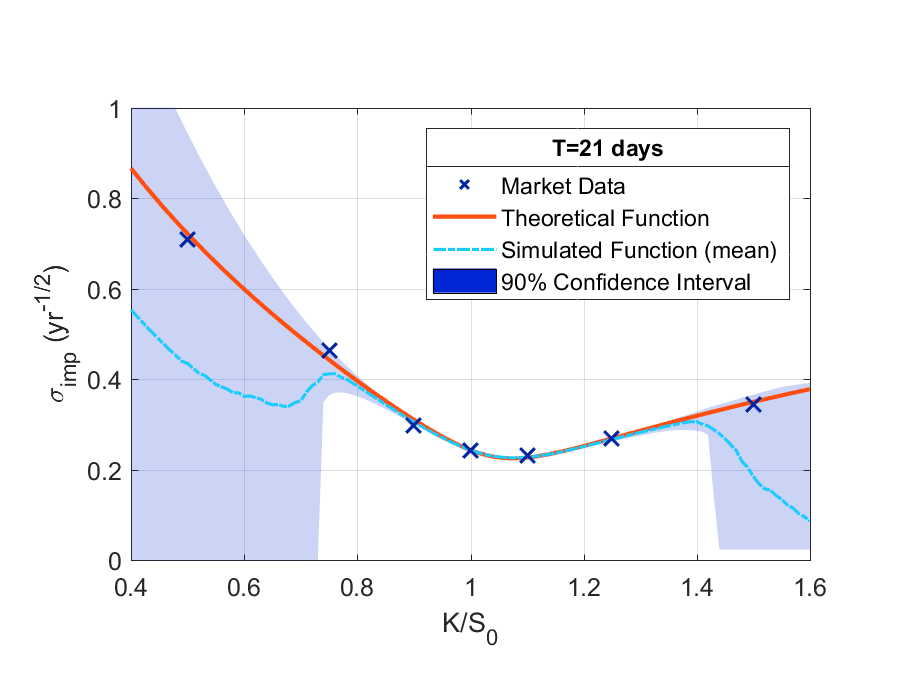
\includegraphics[width=0.49\linewidth,trim={0.25cm 0.45cm 1.1cm 1.4cm},clip]{SSABR1.eps}}
    \subfigure[$T=42$ days]{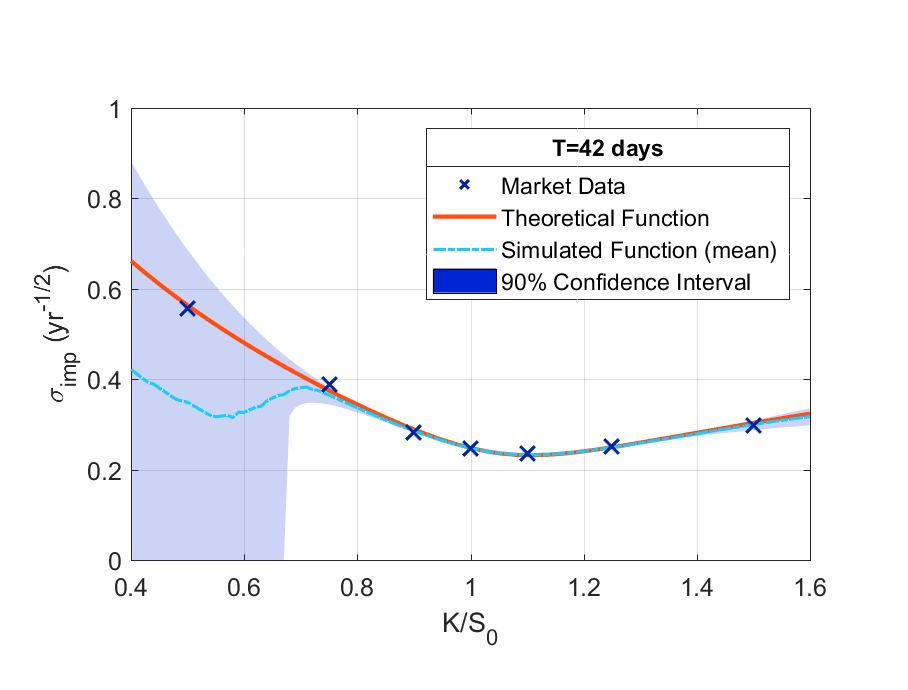
\includegraphics[width=0.49\linewidth,trim={0.25cm 0.45cm 1.1cm 1.4cm},clip]{SSABR2.eps}}
    \subfigure[$T=63$ days]{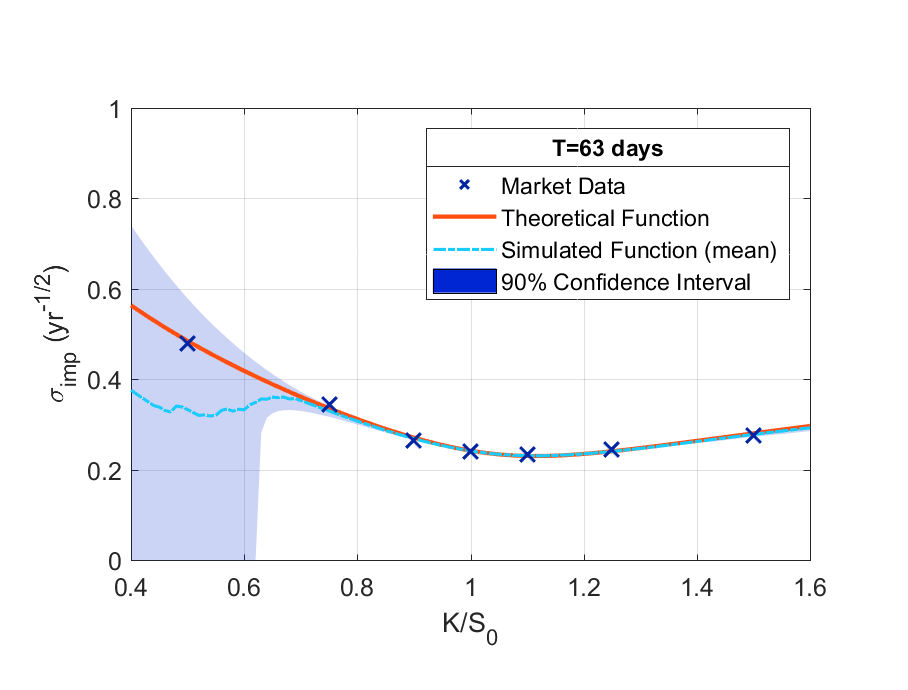
\includegraphics[width=0.49\linewidth,trim={0.25cm 0.45cm 1.1cm 1.4cm},clip]{SSABR3.eps}}
    \subfigure[$T=126$ days]{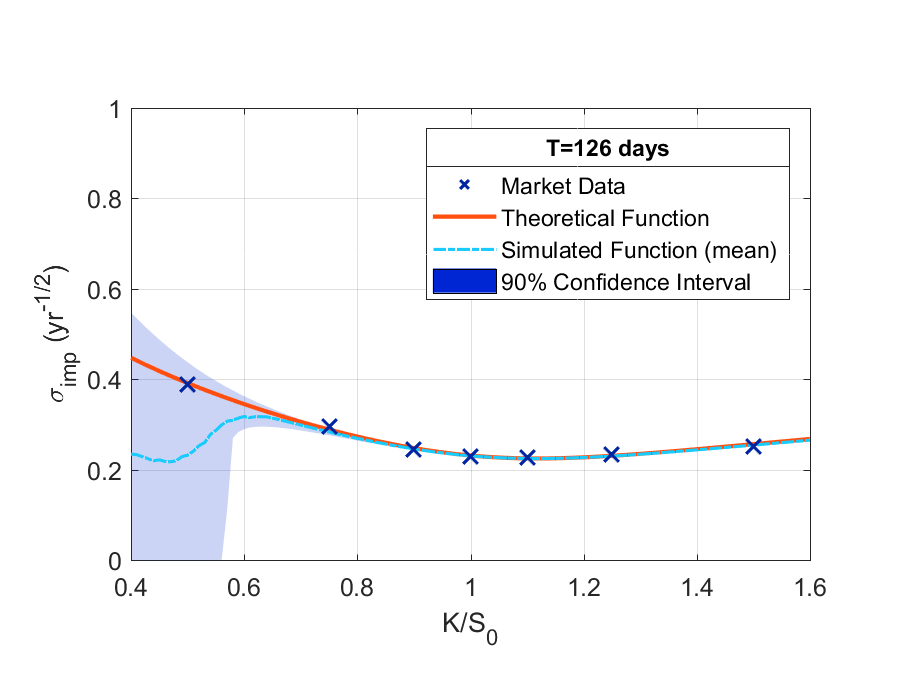
\includegraphics[width=0.49\linewidth,trim={0.25cm 0.45cm 1.1cm 1.4cm},clip]{SSABR4.eps}}
  \end{subfigmatrix}
  \caption[Implied volatility functions fitted independently to the implied volatility data for different maturities under the static SABR model, plotted with their respective Monte Carlo simulated functions along with their 90\% confidence intervals.]{Implied volatility functions (red lines) fitted independently to the implied volatility data (crosses) for different maturities under the static SABR model, plotted with their respective Monte Carlo simulated functions (light-blue dot-dashed lines) along with their 90\% confidence intervals (blue region).}
  \label{fig:SS}
\end{figure}


\begin{table}[H]
    \centering
        \renewcommand{\arraystretch}{0.8}
\begin{tabular}{@{}lccccr@{}}
\toprule
 $T$(days) & $\alpha$ ($\SI{}{\year\tothe{-1/2}}$) & $\beta$ & $\rho$ & $\nu$ & Cost \\ \midrule
21 & 0.2381 & 0.3766 & -0.3760 & 2.1022 & 0.000415 \\
42 & 0.2434 & 0.7362 & -0.3664 & 1.4451 & 0.000166\\
63 & 0.2375 & 0.7750 & -0.3119 & 1.1420 & 0.000102\\
126& 0.2267 & 0.8771 & -0.2383 & 0.8215 & 0.000055\\
\bottomrule
\end{tabular}
  \caption[Fitted parameters for each maturity (fitted independently) under static SABR model.]{Fitted parameters for each maturity (fitted independently) under static SABR model.}
  \label{tab:SSR}
\end{table}


\begin{table}[H]
\centering
\renewcommand{\arraystretch}{0.8}
\begin{tabular}{@{}lccccccr@{}}
\toprule
$T$(days) & $K$($\EUR$) & $\sigma_{i,\mathrm{mkt}}$($\SI{}{\year\tothe{-1/2}}$) &  $\sigma_{i,\mathrm{mdl}}$($\SI{}{\year\tothe{-1/2}}$) &$\mathrm{Error}_{\sigma}(\%)$&$C_{\mathrm{mkt}}$($\EUR$)&$C_{\mathrm{mdl}}$($\EUR$)& $\mathrm{Error}_{C}(\%)$\\ \midrule
\multirow{7}{*}{21} & 0.50 & 0.7082 & 0.7209 & 1.8 & 0.50001 & 0.50002 & 0.001 \\
&0.75 & 0.4632 & 0.4428 & 4.4 & 0.25065 & 0.25047 & 0.1 \\
&0.90 & 0.2989 & 0.3105 & 3.9 & 0.10439 & 0.10501 & 0.6 \\
&1.00 & 0.2425 & 0.2435 & 0.4 & 0.02792 & 0.02804 & 0.4 \\
&1.10 & 0.2314 & 0.2269 & 2.0 & 2.42$\times10^{-3}$ & 2.23$\times10^{-3}$ & 8.0 \\
&1.25 & 0.2699 & 0.2692 & 0.3 & 5.34$\times10^{-5}$ & 5.18$\times10^{-5}$ & 3.0 \\
&1.50 & 0.3433 & 0.3500 & 1.9 & 5.75$\times10^{-7}$ & 8.32$\times10^{-7}$ & 44.7 \\\midrule
\multirow{7}{*}{42} &0.50 & 0.5556 & 0.5631 & 1.4 & 0.50005 & 0.50006 & 0.002 \\
&0.75 & 0.3876 & 0.3751 & 3.2 & 0.25186 & 0.25155 & 0.1 \\
&0.90 & 0.2824 & 0.2891 & 2.4 & 0.11069 & 0.11139 & 0.6 \\
&1.00 & 0.2461 & 0.2481 & 0.8 & 0.04006 & 0.04039 & 0.8 \\
&1.10 & 0.2354 & 0.2322 & 1.4 & 8.52$\times10^{-3}$ & 8.19$\times10^{-3}$ & 3.9 \\
&1.25 & 0.2525 & 0.2497 & 1.1 & 6.21$\times10^{-4}$ & 5.75$\times10^{-4}$ & 7.4 \\
&1.50 & 0.2968 & 0.3033 & 2.2 & 1.58$\times10^{-5}$ & 2.12$\times10^{-5}$ & 33.9 \\\midrule
\multirow{7}{*}{63} &0.50 & 0.4789 & 0.4845 & 1.2 & 0.50009 & 0.50011 & 0.002 \\
&0.75 & 0.3452 & 0.3357 & 2.8 & 0.25296 & 0.25256 & 0.2 \\
&0.90 & 0.2658 & 0.2710 & 2.0 & 0.11533 & 0.11605 & 0.6 \\
&1.00 & 0.2401 & 0.2421 & 0.8 & 0.04787 & 0.04826 & 0.8 \\
&1.10 & 0.2330 & 0.2305 & 1.1 & 0.01421 & 0.01384 & 2.6 \\
&1.25 & 0.2438 & 0.2409 & 1.2 & 1.80$\times10^{-3}$ & 1.68$\times10^{-3}$ & 6.7 \\
&1.50 & 0.2749 & 0.2804 & 2.0 & 7.66$\times10^{-5}$ & 9.56$\times10^{-5}$ & 24.8 \\\midrule
\multirow{7}{*}{126} &0.50 & 0.3878 & 0.3914 & 0.9 & 0.50035 & 0.50038 & 0.006 \\
&0.75 & 0.2954 & 0.2887 & 2.2 & 0.25694 & 0.25633 & 0.2 \\
&0.90 & 0.2444 & 0.2479 & 1.5 & 0.12716 & 0.12794 & 0.6 \\
&1.00 & 0.2295 & 0.2314 & 0.8 & 0.06467 & 0.06522 & 0.8 \\
&1.10 & 0.2269 & 0.2251 & 0.8 & 0.02862 & 0.02817 & 1.6 \\
&1.25 & 0.2340 & 0.2309 & 1.3 & 7.57$\times10^{-3}$ & 7.18$\times10^{-3}$ & 5.2 \\
&1.50 & 0.2521 & 0.2567 & 1.8 & 8.58$\times10^{-4}$ & 9.82$\times10^{-4}$ & 14.5 \\
 \bottomrule
\end{tabular}
  \caption[Comparison between fitted results and original data under static SABR model.]{Comparison between fitted results and original data under static SABR model.}
  \label{tab:SS}
\end{table}







\newpage
\section{Heston Model}
The Heston model is defined as
\begin{equation}
dS=rSdt+\sqrt{\nu}SdW_1,
\end{equation}
\begin{equation}
d\nu=\kappa(\overline{\nu}-\nu)dt+\eta\sqrt{\nu}dW_2,
\end{equation}
\noindent where $\nu_0=\nu(0)$ and with $W_1$ and $W_2$ having a correlation of $\rho$.

The closed form solution, shown in eq.\eqref{CH}, we are able to find the theoretical prices of options priced under this model, which we can easily convert to implied volatilities. These last will be used in the calibration process.

The influence of each parameter of the Heston model on the shape of the implied volatility curve is shown in \autoref{fig:Hparam}.

\begin{figure}[H]
  \begin{subfigmatrix}{2}
    \subfigure[Dependence on $\kappa$]{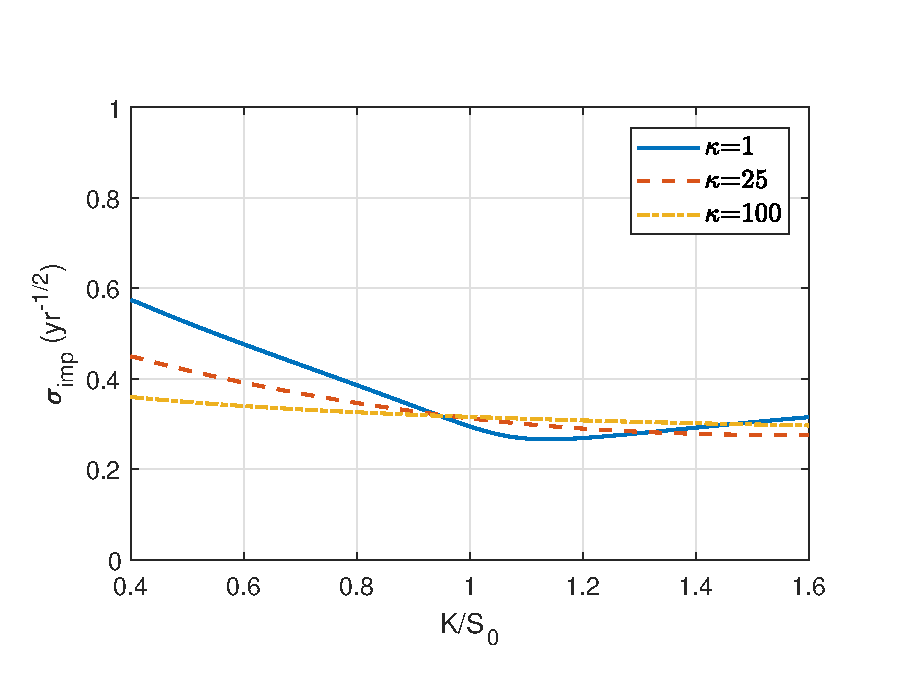
\includegraphics[width=0.49\linewidth,trim={0.25cm 0.45cm 1.1cm 1.4cm},clip]{Hkappa.eps}}
    \subfigure[Dependence on $\overline{\nu}$]{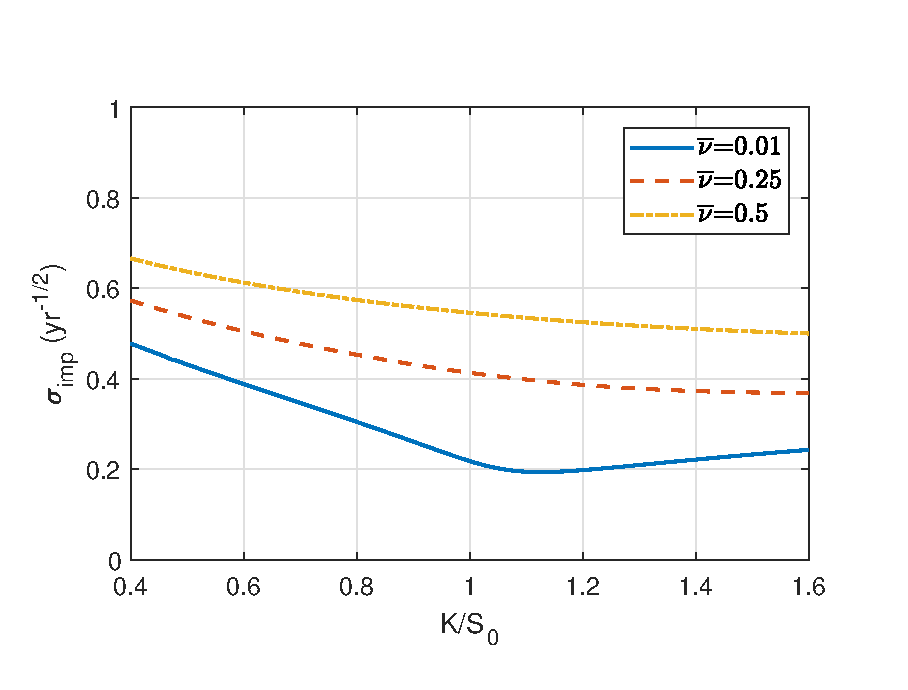
\includegraphics[width=0.49\linewidth,trim={0.25cm 0.45cm 1.1cm 1.4cm},clip]{Hnubar.eps}}
    \subfigure[Dependence on $\nu_0$]{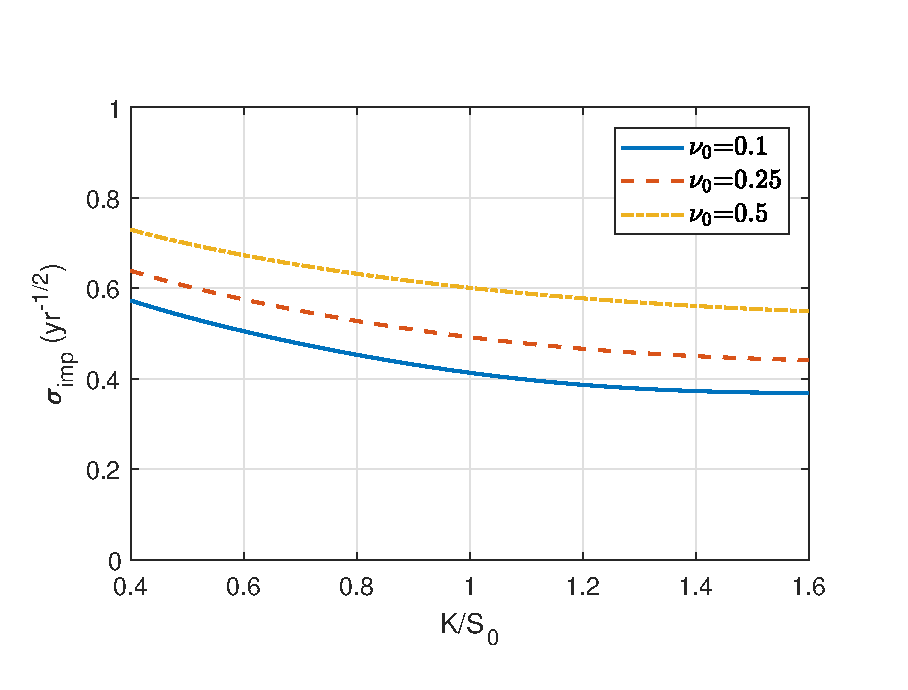
\includegraphics[width=0.49\linewidth,trim={0.25cm 0.45cm 1.1cm 1.4cm},clip]{Hnu0.eps}}
    \subfigure[Dependence on $\eta$]{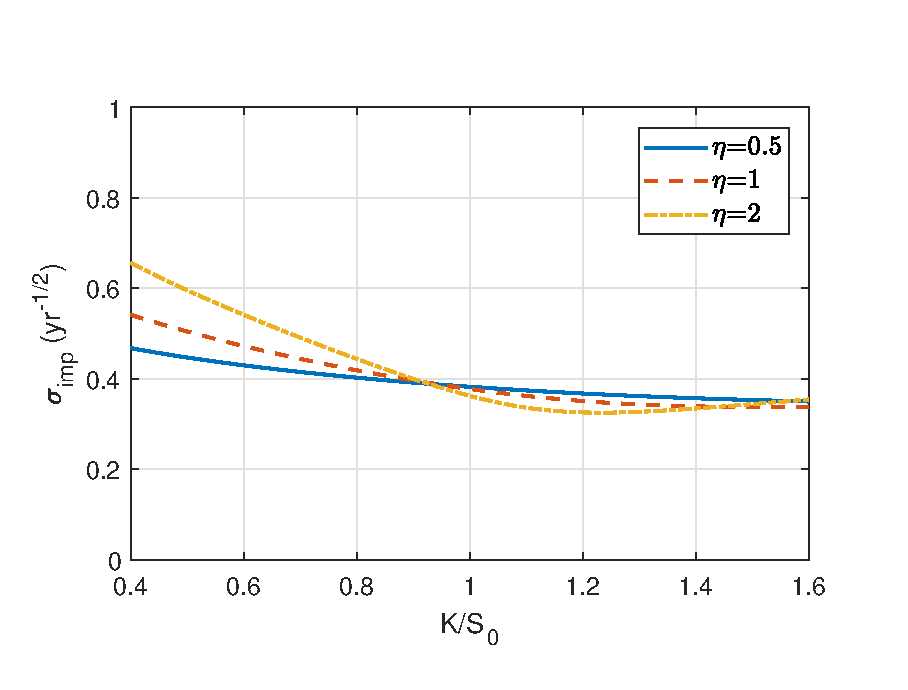
\includegraphics[width=0.49\linewidth,trim={0.25cm 0.45cm 1.1cm 1.4cm},clip]{Heta.eps}}
        \subfigure[Dependence on $\rho$]{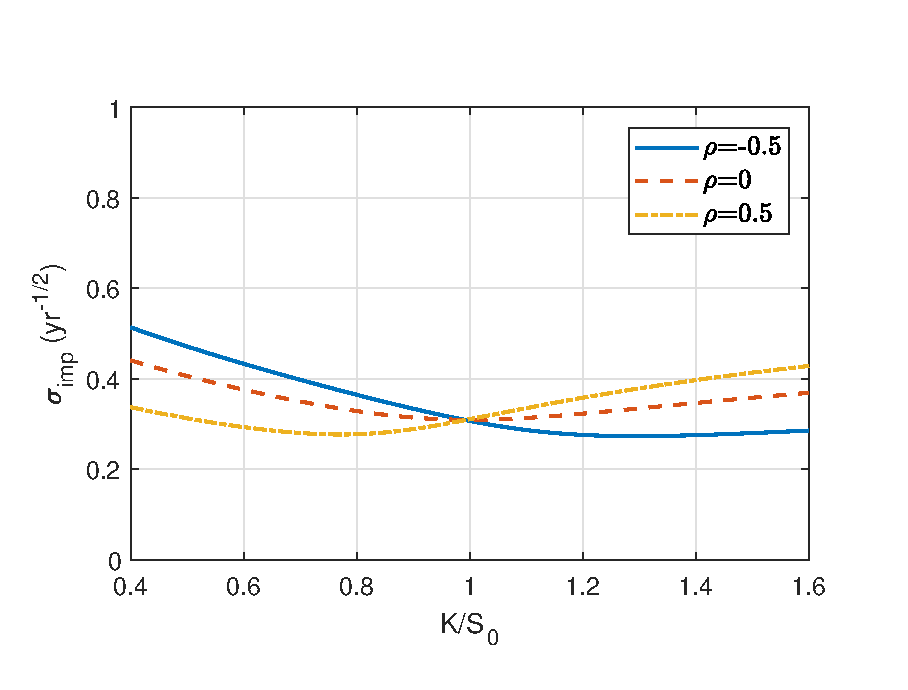
\includegraphics[width=0.49\linewidth,trim={0.25cm 0.45cm 1.1cm 1.4cm},clip]{Hrho.eps}}
  \end{subfigmatrix}
  \caption[Dependence of the implied volatility curve on each of the Heston model parameters.]{Dependence of the implied volatility curve on each of the Heston model parameters. The default parameters used were $S_0=1\EUR$, $T=42$ days and $r=0$. Furthermore, on all plots, except when the dependence on a parameter is represented, the parameters used were $\kappa=10$, $\overline{\nu}=0.1$, $\nu_0=0.1$, $\eta=1$ and $\rho=-0.5$.}
  \label{fig:Hparam}
\end{figure}


\begin{figure}[H]
  \begin{subfigmatrix}{2}
    \subfigure[$T=21$ days]{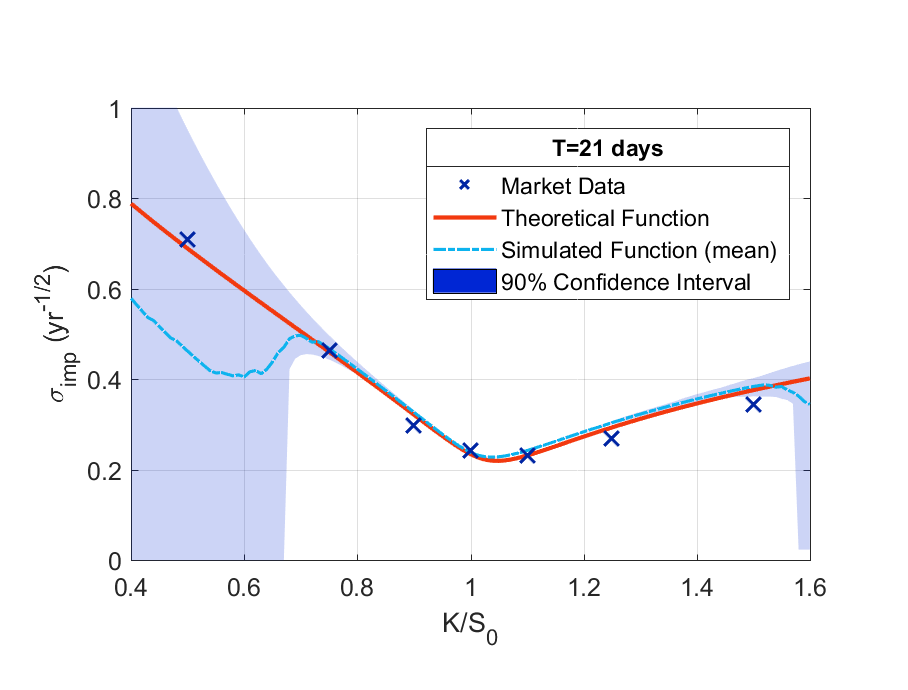
\includegraphics[width=0.49\linewidth,trim={0.25cm 0.45cm 1.1cm 1.4cm},clip]{H1.eps}}
    \subfigure[$T=42$ days]{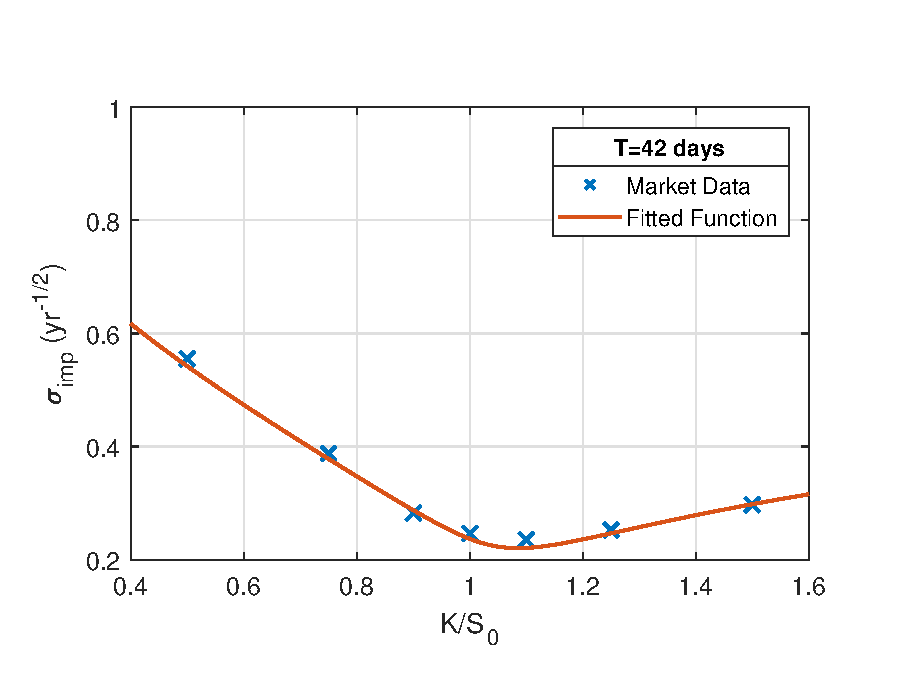
\includegraphics[width=0.49\linewidth,trim={0.25cm 0.45cm 1.1cm 1.4cm},clip]{H2.eps}}
    \subfigure[$T=63$ days]{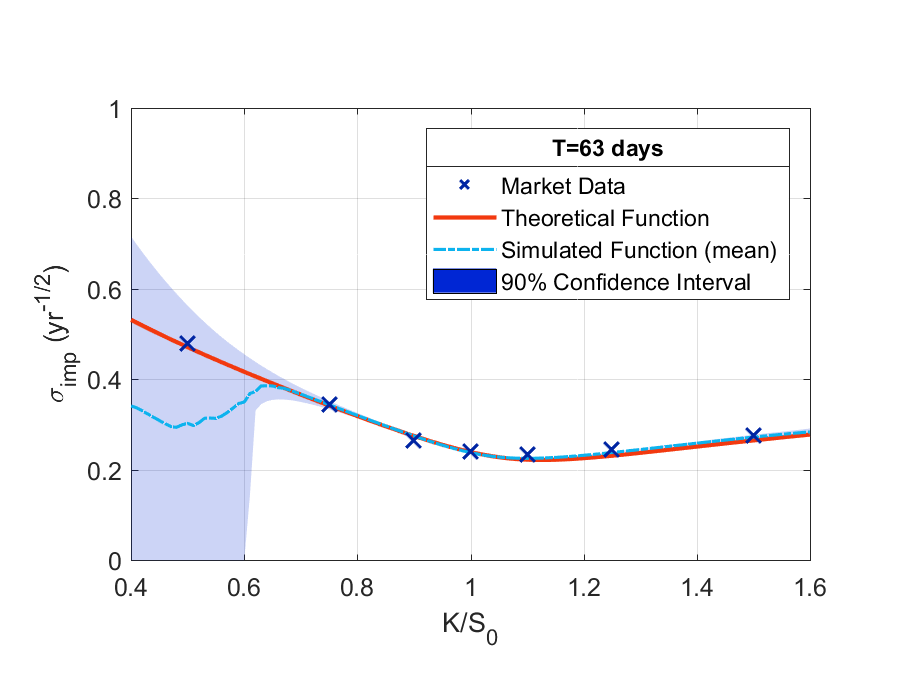
\includegraphics[width=0.49\linewidth,trim={0.25cm 0.45cm 1.1cm 1.4cm},clip]{H3.eps}}
    \subfigure[$T=126$ days]{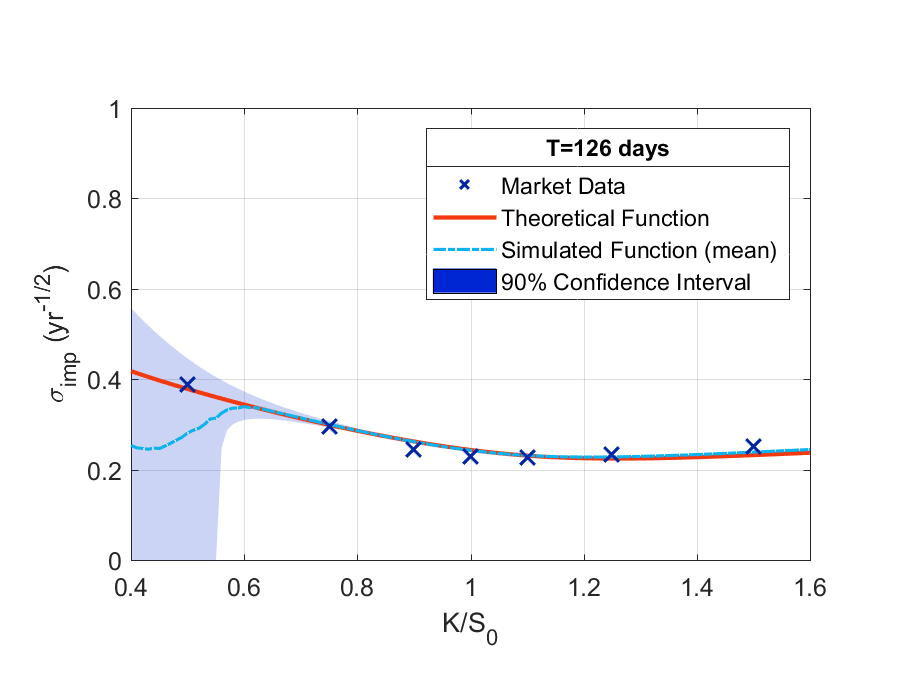
\includegraphics[width=0.49\linewidth,trim={0.25cm 0.45cm 1.1cm 1.4cm},clip]{H4.eps}}
  \end{subfigmatrix}
  \caption[Implied volatility functions fitted simultaneously to the implied volatility data for different maturities under the Heston model, plotted with their respective Monte Carlo simulated functions along with their 90\% confidence intervals.]{Implied volatility functions (red lines) fitted simultaneously to the implied volatility data (crosses) for different maturities under the Heston model, plotted with their respective Monte Carlo simulated functions (light-blue dot-dashed lines) along with their 90\% confidence intervals (blue region).}
  \label{fig:H}
\end{figure}




\begin{figure}[H]
  \begin{subfigmatrix}{2}
    \subfigure[$\sigma_{imp}$ surface]{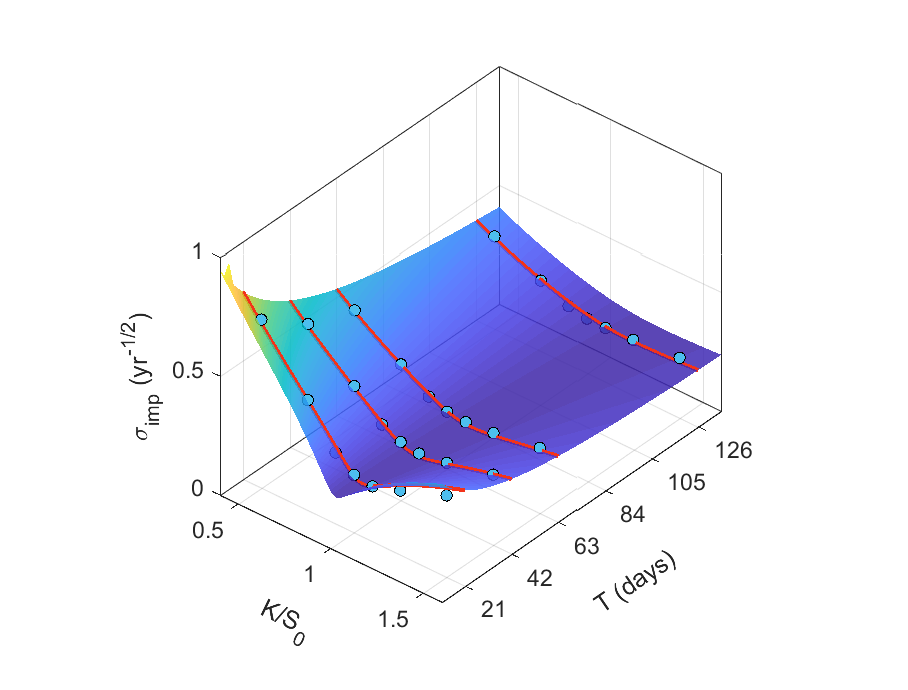
\includegraphics[width=0.49\linewidth,trim={1.7cm 0.45cm 2.35cm 0.85cm},clip]{HS.eps}}
    \subfigure[$\sigma_{imp}$ contour plot]{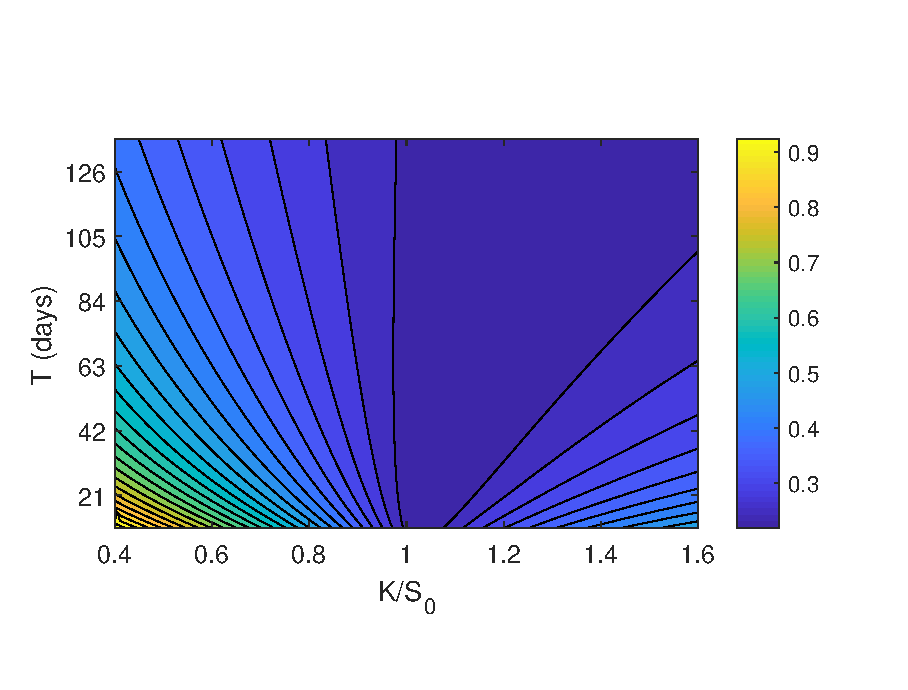
\includegraphics[width=0.49\linewidth,trim={0.2cm 0.5cm 1.25cm 1.55cm},clip]{HSC.eps}}
  \end{subfigmatrix}
    \caption[Implied volatility surface and corresponding contour plot of the function fitted simmultaneously to the implied volatility data for different maturities under the Heston model, plotted against the original market data and the fitted functions shown in \autoref{fig:H}.]{Implied volatility surface (left) and corresponding contour plot (right) of the function fitted simmultaneously to the implied volatility data for different maturities under the Heston model, plotted against the original market data (blue circles) and the fitted functions shown in \autoref{fig:H} (red lines).}\label{fig:HS}
\end{figure}   


\begin{figure}[H]
  \begin{subfigmatrix}{2}
    \subfigure[$\sigma_{imp}$ surface]{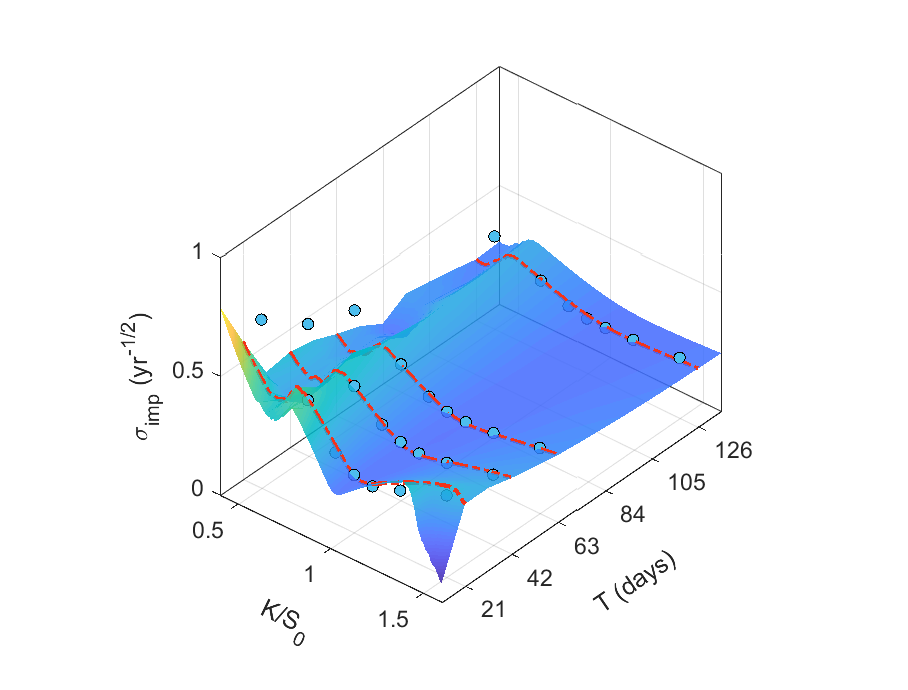
\includegraphics[width=0.49\linewidth,trim={1.7cm 0.45cm 2.35cm 0.85cm},clip]{HSSim.eps}}
    \subfigure[$\sigma_{imp}$ contour plot]{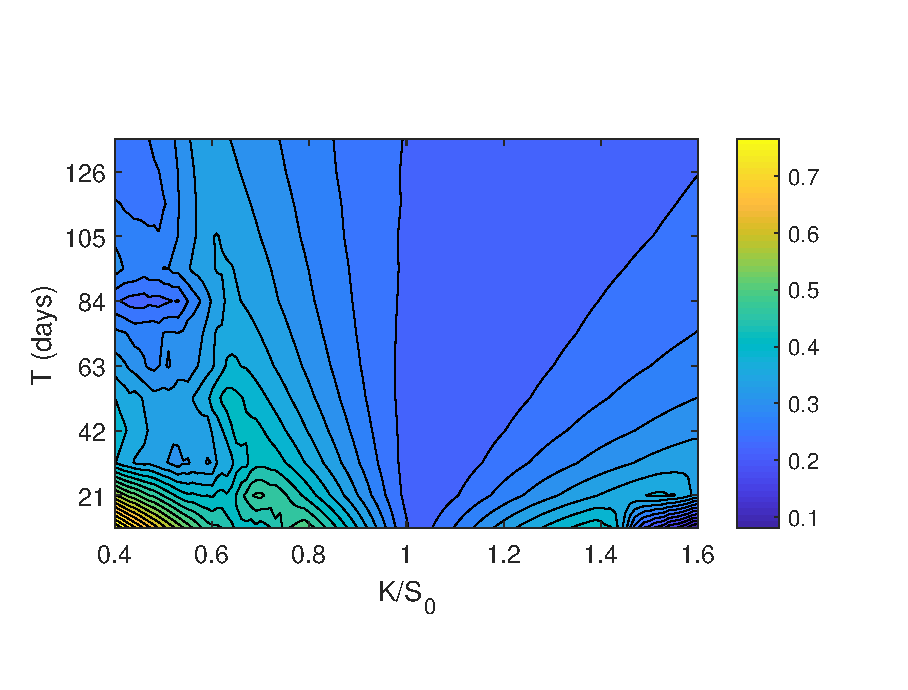
\includegraphics[width=0.49\linewidth,trim={0.2cm 0.5cm 1.25cm 1.55cm},clip]{HSCSim.eps}}
  \end{subfigmatrix}
    \caption[Implied volatility surface and corresponding contour plot of the function simulated using the Monte Carlo procedure with the fitted parameters shown in \autoref{tab:HR}, under the Heston model, plotted against the original market data and the simulated functions shown in \autoref{fig:H}.]{Implied volatility surface (left) and corresponding contour plot (right) of the function simulated using the Monte Carlo procedure with the fitted parameters shown in \autoref{tab:HR}, under the dynamic SABR model, plotted against the original market data (blue circles) and the simulated functions shown in \autoref{fig:H} (red dot-dashed lines).}\label{fig:HSSim}
\end{figure} 



\begin{table}[H]
    \centering
        \renewcommand{\arraystretch}{0.8}
\begin{tabular}{@{}lccccr@{}}
\toprule
$\kappa$ & $\overline{\nu}$ & $\nu_0$ & $\rho$ & $\eta$ & Cost \\ \midrule
53.4355 & 0.0653 & 0.1046 & -0.4086 & 6.2554 & 0.002529 \\
\bottomrule
\end{tabular}
  \caption[Fitted parameters for all maturities (fitted simultaneously) under the Heston model.]{Fitted parameters for all maturities (fitted simultaneously) under the Heston model.}
  \label{tab:HR}
\end{table}


\begin{table}[H]
\centering
\renewcommand{\arraystretch}{0.8}
\begin{tabular}{@{}lccccccr@{}}
\toprule
$T$(days) & $K$($\EUR$) & $\sigma_{i,\mathrm{mkt}}$($\SI{}{\year\tothe{-1/2}}$) &  $\sigma_{i,\mathrm{mdl}}$($\SI{}{\year\tothe{-1/2}}$) &$\mathrm{Error}_{\sigma}(\%)$&$C_{\mathrm{mkt}}$($\EUR$)&$C_{\mathrm{mdl}}$($\EUR$)& $\mathrm{Error}_{C}(\%)$\\ \midrule
\multirow{7}{*}{21} & 0.50 & 0.7082 & 0.6886 & 2.8 & 0.50001 & 0.50001 & 0.001 \\
 & 0.75 & 0.4632 & 0.4604 & 0.6 & 0.25065 & 0.25062 & 0.01 \\
 & 0.90 & 0.2989 & 0.3216 & 7.6 & 0.10439 & 0.10563 & 1.2 \\
 & 1.00 & 0.2425 & 0.2346 & 3.2 & 0.02792 & 0.02702 & 3.2 \\
 & 1.10 & 0.2314 & 0.2316 & 0.1 & 2.42$\times10^{-3}$ & 2.43$\times10^{-3}$ & 0.3 \\
 & 1.25 & 0.2699 & 0.2935 & 8.7 & 5.34$\times10^{-5}$ & 12.43$\times10^{-5}$ & 132.5 \\
 & 1.50 & 0.3433 & 0.3759 & 9.5 & 5.75$\times10^{-7}$ & 29.58$\times10^{-7}$ & 414.7 \\\midrule
\multirow{7}{*}{42} & 0.50 & 0.5556 & 0.5422 & 2.4 & 0.50005 & 0.50004 & 0.003 \\
 & 0.75 & 0.3876 & 0.3781 & 2.5 & 0.25186 & 0.25162 & 0.1 \\
 & 0.90 & 0.2824 & 0.2873 & 1.7 & 0.11069 & 0.11120 & 0.5 \\
 & 1.00 & 0.2461 & 0.2366 & 3.9 & 0.04006 & 0.03852 & 3.9 \\
 & 1.10 & 0.2354 & 0.2205 & 6.3 & 8.52$\times10^{-3}$ & 7.02$\times10^{-3}$ & 17.6 \\
 & 1.25 & 0.2525 & 0.2463 & 2.4 & 6.21$\times10^{-4}$ & 5.20$\times10^{-4}$ & 16.2 \\
 & 1.50 & 0.2968 & 0.2979 & 0.4 & 1.58$\times10^{-5}$ & 1.66$\times10^{-5}$ & 4.9 \\\midrule
\multirow{7}{*}{63} & 0.50 & 0.4789 & 0.4709 & 1.7 & 0.50009 & 0.50008 & 0.003 \\
 & 0.75 & 0.3452 & 0.3420 & 0.9 & 0.25296 & 0.25282 & 0.1 \\
 & 0.90 & 0.2658 & 0.2748 & 3.4 & 0.11533 & 0.11659 & 1.1 \\
 & 1.00 & 0.2401 & 0.2392 & 0.4 & 0.04787 & 0.04768 & 0.4 \\
 & 1.10 & 0.2330 & 0.2224 & 4.6 & 0.01421 & 0.01265 & 11.0 \\
 & 1.25 & 0.2438 & 0.2310 & 5.2 & 1.80$\times10^{-3}$ & 1.31$\times10^{-3}$ & 27.1 \\
 & 1.50 & 0.2749 & 0.2649 & 3.7 & 7.66$\times10^{-5}$ & 4.97$\times10^{-5}$ & 35.1 \\\midrule
\multirow{7}{*}{126} & 0.50 & 0.3878 & 0.3784 & 2.4 & 0.50035 & 0.50028 & 0.01 \\
 & 0.75 & 0.2954 & 0.2993 & 1.3 & 0.25694 & 0.25732 & 0.1 \\
 & 0.90 & 0.2444 & 0.2626 & 7.5 & 0.12716 & 0.13124 & 3.2 \\
 & 1.00 & 0.2295 & 0.2439 & 6.3 & 0.06467 & 0.06870 & 6.2 \\
 & 1.10 & 0.2269 & 0.2314 & 2.0 & 0.02862 & 0.02973 & 3.9 \\
 & 1.25 & 0.2340 & 0.2248 & 3.9 & 7.57$\times10^{-3}$ & 6.45$\times10^{-3}$ & 14.8 \\
 & 1.50 & 0.2521 & 0.2324 & 7.8 & 8.58$\times10^{-4}$ & 4.45$\times10^{-4}$ & 48.2 \\ 
 \bottomrule
\end{tabular}
  \caption[Comparison between fitted results and original data under the Heston model.]{Comparison between fitted results and original data under the Heston model.}
  \label{tab:H}
\end{table}











\newpage

\section{Dynamic SABR Model}
\begin{figure}[H]
  \begin{subfigmatrix}{2}
    \subfigure[$T=21$ days]{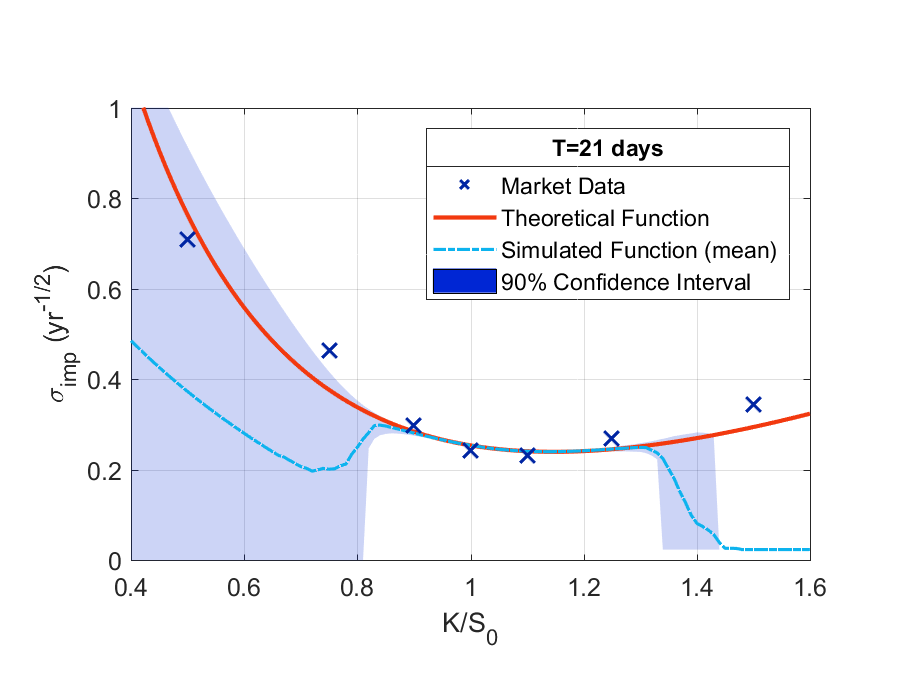
\includegraphics[width=0.49\linewidth,trim={0.25cm 0.45cm 1.1cm 1.4cm},clip]{DS1.eps}}
    \subfigure[$T=42$ days]{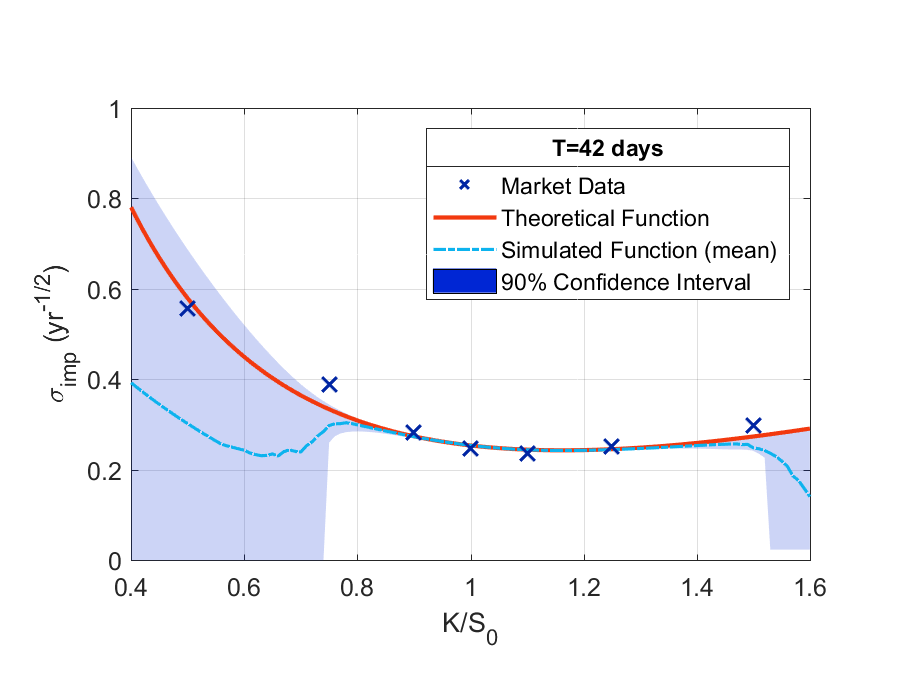
\includegraphics[width=0.49\linewidth,trim={0.25cm 0.45cm 1.1cm 1.4cm},clip]{DS2.eps}}
    \subfigure[$T=63$ days]{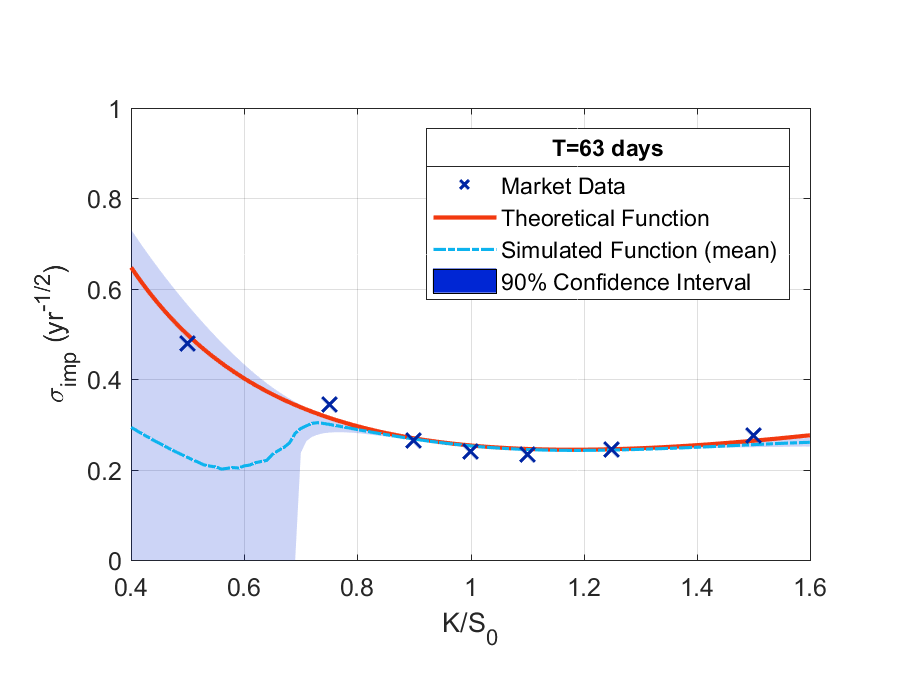
\includegraphics[width=0.49\linewidth,trim={0.25cm 0.45cm 1.1cm 1.4cm},clip]{DS3.eps}}
    \subfigure[$T=126$ days]{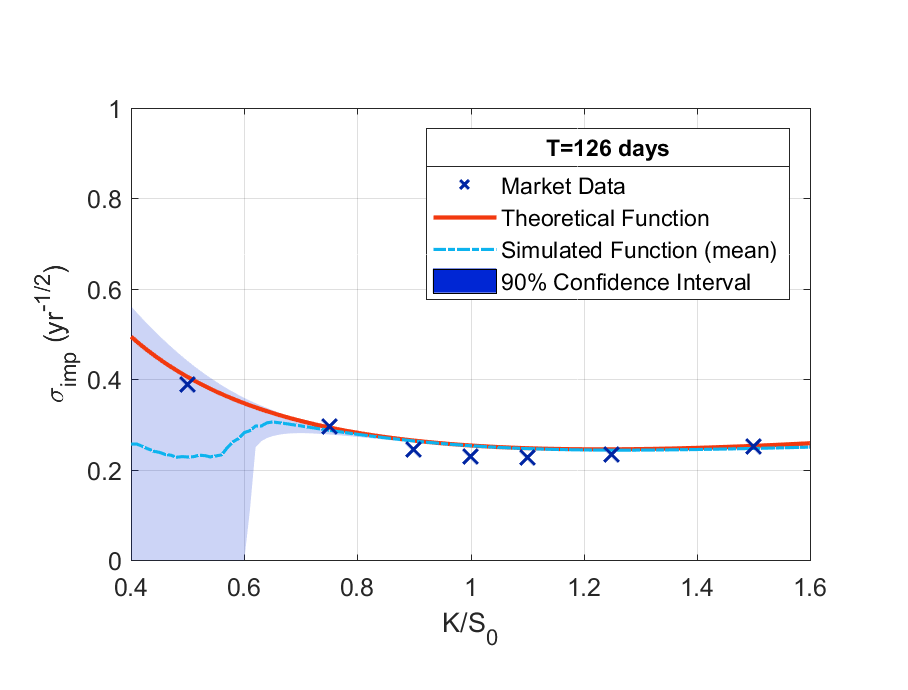
\includegraphics[width=0.49\linewidth,trim={0.25cm 0.45cm 1.1cm 1.4cm},clip]{DS4.eps}}
  \end{subfigmatrix}
  \caption[Implied volatility functions fitted simultaneously to the implied volatility data for different maturities under the dynamic SABR model, plotted with their respective Monte Carlo simulated functions along with their 90\% confidence intervals.]{Implied volatility functions (red lines) fitted simultaneously to the implied volatility data (crosses) for different maturities under the dynamic SABR model, plotted with their respective Monte Carlo simulated functions (light-blue dot-dashed lines) along with their 90\% confidence intervals (blue region).}
  \label{fig:DS}
\end{figure}


\begin{figure}[H]
  \begin{subfigmatrix}{2}
    \subfigure[$\sigma_{imp}$ surface]{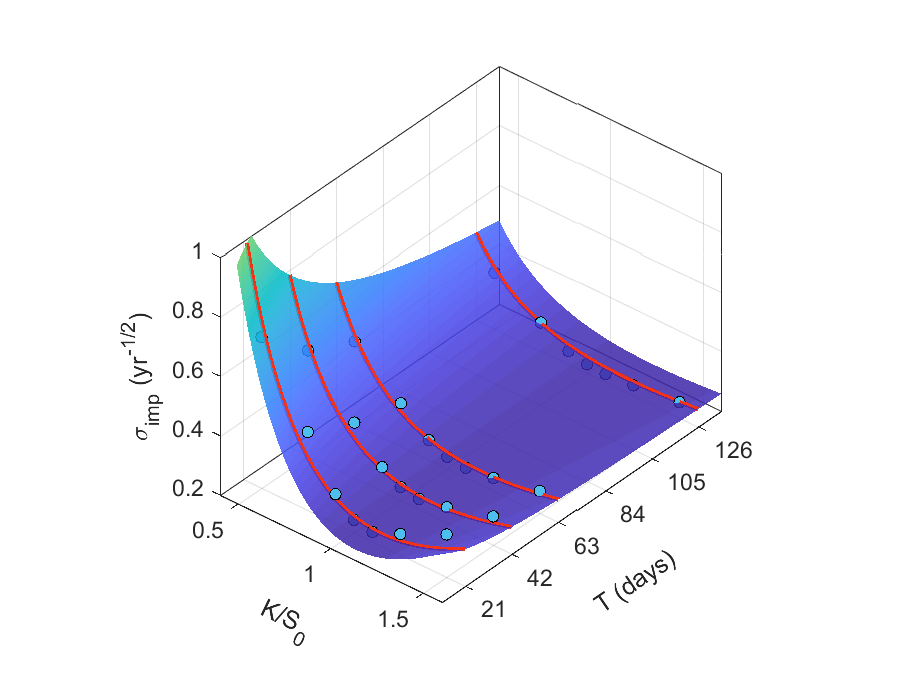
\includegraphics[width=0.49\linewidth,trim={1.7cm 0.45cm 2.35cm 0.85cm},clip]{DSS.eps}}
    \subfigure[$\sigma_{imp}$ contour plot]{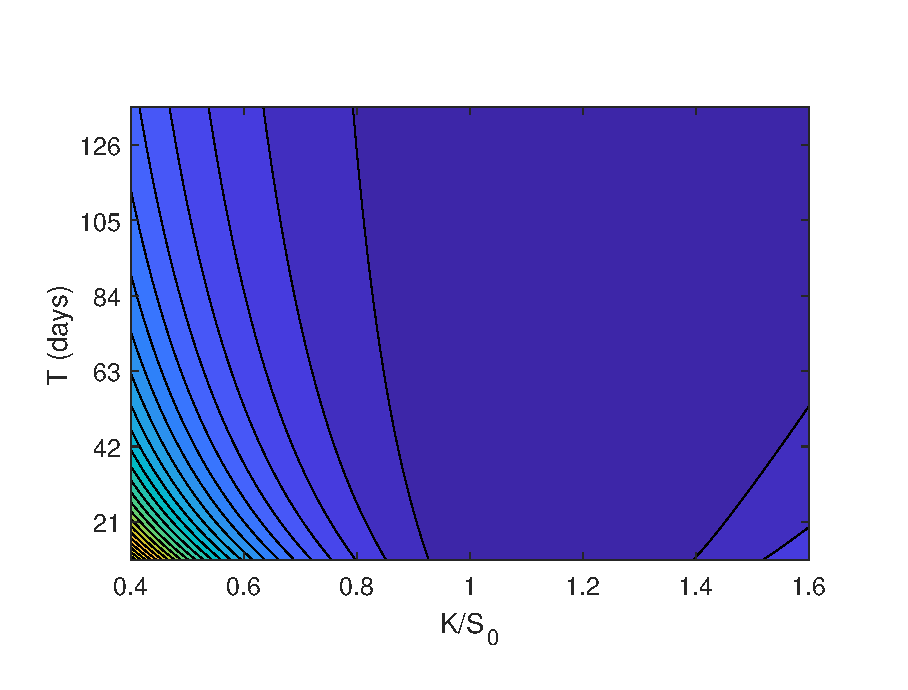
\includegraphics[width=0.49\linewidth,trim={0.2cm 0.5cm 1.25cm 1.55cm},clip]{DSSC.eps}}
  \end{subfigmatrix}
    \caption[Implied volatility surface and corresponding contour plot of the function fitted simmultaneously to the implied volatility data for different maturities under the dynamic SABR model, plotted against the original market data and the fitted functions shown in \autoref{fig:DS}.]{Implied volatility surface (left) and corresponding contour plot (right) of the function fitted simmultaneously to the implied volatility data for different maturities under the dynamic SABR model, plotted against the original market data (blue circles) and the fitted functions shown in \autoref{fig:DS} (red lines).}\label{fig:DSS}
\end{figure}   



\begin{figure}[H]
  \begin{subfigmatrix}{2}
    \subfigure[$\sigma_{imp}$ surface]{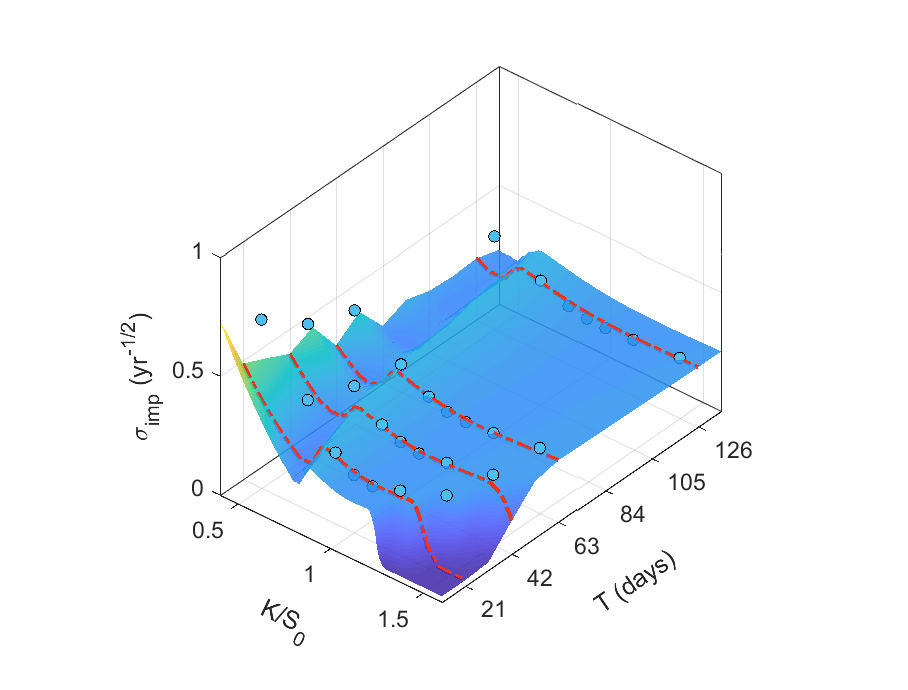
\includegraphics[width=0.49\linewidth,trim={1.7cm 0.45cm 2.35cm 0.85cm},clip]{DSSSim.eps}}
    \subfigure[$\sigma_{imp}$ contour plot]{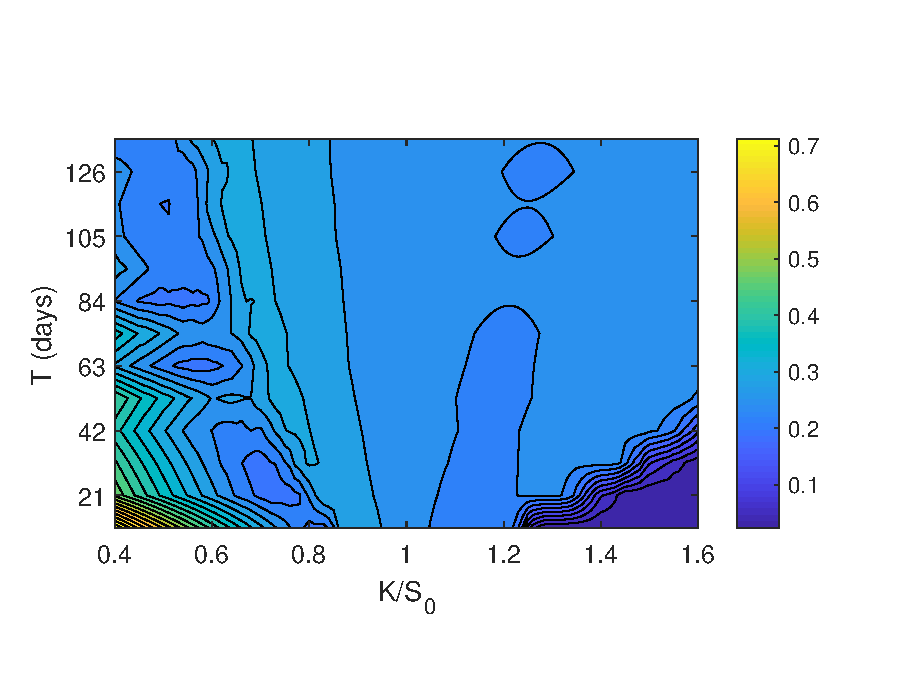
\includegraphics[width=0.49\linewidth,trim={0.2cm 0.5cm 1.25cm 1.55cm},clip]{DSSCSim.eps}}
  \end{subfigmatrix}
    \caption[Implied volatility surface and corresponding contour plot of the function simulated using the Monte Carlo procedure with the fitted parameters shown in \autoref{tab:DSR}, under the dynamic SABR model, plotted against the original market data and the simulated functions shown in \autoref{fig:DS}.]{Implied volatility surface (left) and corresponding contour plot (right) of the function simulated using the Monte Carlo procedure with the fitted parameters shown in \autoref{tab:DSR}, under the dynamic SABR model, plotted against the original market data (blue circles) and the simulated functions shown in \autoref{fig:DS} (red dot-dashed lines).}\label{fig:DSSSim}
\end{figure} 


\begin{table}[H]
    \centering
        \renewcommand{\arraystretch}{0.8}
\begin{tabular}{@{}lcccccr@{}}
\toprule
$\alpha$ & $\beta$ & $\rho_0$ & $a$ & $\nu_0$ & $b$ & Cost \\ \midrule
0.2540 & 0.6348 & -0.4166 & 0 & 1.8673 & 41.6943 & 0.0108 \\
\bottomrule
\end{tabular}
  \caption[Fitted parameters for all maturities (fitted simultaneously) under the dynamic SABR model.]{Fitted parameters for all maturities (fitted simultaneously) under the dynamic SABR model.}
  \label{tab:DSR}
\end{table}


\begin{table}[H]
\centering
\renewcommand{\arraystretch}{0.8}
\begin{tabular}{@{}lccccccr@{}}
\toprule
$T$(days) & $K$($\EUR$) & $\sigma_{i,\mathrm{mkt}}$($\SI{}{\year\tothe{-1/2}}$) &  $\sigma_{i,\mathrm{mdl}}$($\SI{}{\year\tothe{-1/2}}$) &$\mathrm{Error}_{\sigma}(\%)$&$C_{\mathrm{mkt}}$($\EUR$)&$C_{\mathrm{mdl}}$($\EUR$)& $\mathrm{Error}_{C}(\%)$\\ \midrule
\multirow{7}{*}{21} & 0.50 & 0.7082 & 0.7625 & 7.7 & 0.50001 & 0.50003 & 0.004 \\
 & 0.75 & 0.4632 & 0.3765 & 18.7 & 0.25065 & 0.25012 & 0.2 \\
 & 0.90 & 0.2989 & 0.2843 & 4.9 & 0.10439 & 0.10367 & 0.7 \\
 & 1.00 & 0.2425 & 0.2540 & 4.7 & 0.02792 & 0.02924 & 4.7 \\
 & 1.10 & 0.2314 & 0.2410 & 4.2 & 2.42$\times10^{-3}$ & 2.86$\times10^{-3}$ & 18.0 \\
 & 1.25 & 0.2699 & 0.2454 & 9.1 & 5.34$\times10^{-5}$ & 1.76$\times10^{-5}$ & 67.1 \\
 & 1.50 & 0.3433 & 0.2944 & 14.2 & 57.48$\times10^{-8}$ & 1.86$\times10^{-8}$ & 96.8 \\\midrule
\multirow{7}{*}{42} & 0.50 & 0.5556 & 0.5788 & 4.2 & 0.50005 & 0.50008 & 0.01 \\
 & 0.75 & 0.3876 & 0.3337 & 13.9 & 0.25186 & 0.25074 & 0.4 \\
 & 0.90 & 0.2824 & 0.2740 & 3.0 & 0.11069 & 0.10985 & 0.8 \\
 & 1.00 & 0.2461 & 0.2538 & 3.1 & 0.04006 & 0.04131 & 3.1 \\
 & 1.10 & 0.2354 & 0.2445 & 3.9 & 8.52$\times10^{-3}$ & 9.49$\times10^{-3}$ & 11.3 \\
 & 1.25 & 0.2525 & 0.2455 & 2.8 & 6.21$\times10^{-4}$ & 5.07$\times10^{-4}$ & 18.3 \\
 & 1.50 & 0.2968 & 0.2736 & 7.8 & 15.83$\times10^{-6}$ & 4.72$\times10^{-6}$ & 70.2 \\\midrule
\multirow{7}{*}{63} & 0.50 & 0.4789 & 0.4980 & 4.0 & 0.50009 & 0.50014 & 0.01 \\
 & 0.75 & 0.3452 & 0.3150 & 8.8 & 0.25296 & 0.25182 & 0.5 \\
 & 0.90 & 0.2658 & 0.2695 & 1.4 & 0.11533 & 0.11585 & 0.4 \\
 & 1.00 & 0.2401 & 0.2537 & 5.7 & 0.04787 & 0.05057 & 5.6 \\
 & 1.10 & 0.2330 & 0.2460 & 5.6 & 0.01421 & 0.01619 & 13.9 \\
 & 1.25 & 0.2438 & 0.2455 & 0.7 & 1.80$\times10^{-3}$ & 1.87$\times10^{-3}$ & 3.8 \\
 & 1.50 & 0.2749 & 0.2642 & 3.9 & 7.66$\times10^{-5}$ & 4.81$\times10^{-5}$ & 37.2 \\\midrule
\multirow{7}{*}{126} & 0.50 & 0.3878 & 0.4050 & 4.4 & 0.50035 & 0.50051 & 0.03 \\
 & 0.75 & 0.2954 & 0.2935 & 0.6 & 0.25694 & 0.25677 & 0.1 \\
 & 0.90 & 0.2444 & 0.2645 & 8.2 & 0.12716 & 0.13168 & 3.6 \\
 & 1.00 & 0.2295 & 0.2537 & 10.5 & 0.06467 & 0.07147 & 10.5 \\
 & 1.10 & 0.2269 & 0.2477 & 9.1 & 0.02862 & 0.03382 & 18.2 \\
 & 1.25 & 0.2340 & 0.2452 & 4.8 & 7.57$\times10^{-3}$ & 9.05$\times10^{-3}$ & 19.6 \\
 & 1.50 & 0.2521 & 0.2528 & 0.3 & 8.58$\times10^{-4}$ & 8.77$\times10^{-4}$ & 2.3 \\
 \bottomrule
\end{tabular}
  \caption[Comparison between fitted results and original data under the dynamic SABR model.]{Comparison between fitted results and original data under the dynamic SABR model.}
  \label{tab:DS}
\end{table}



\newpage


\hl{check notation:}

$\sigma_{i,\mathrm{mkt}}$ vs $\sigma_{imp,\mathrm{mkt}}$;

\hl{should we include the market values in all comparison tables?}

\hl{put units in fitted parameters}

\hl{is implied vol measured in yr-1/2}

\hl{the heston and dynamic sabr single plot figures are slices of the implied volatility surface}

\hl{talk about the problem of volatility with sabr (switch volatility and price in code)}

\hl{plot the decaying functions of rho and nu on the dynamic sabr model}

\hl{mention the parameters used to simulate each monte carlo pricer}

\hl{mention sabr negative vol is not problematic}

\hl{in the background plots (and implementation), use dashed and dot-dashed lines}

\hl{in the results section, the dashed lines look not-dashed}

\hl{align values in tables}